% arara: xelatex
% arara: xelatex
% arara: xelatex


% options:
% thesis=B bachelor's thesis
% thesis=M master's thesis
% czech thesis in Czech language
% english thesis in English language
% hidelinks remove colour boxes around hyperlinks

\documentclass[thesis=B,english]{FITthesis}[2012/10/20]

\usepackage[utf8]{inputenc} % LaTeX source encoded as UTF-8
% \usepackage[latin2]{inputenc} % LaTeX source encoded as ISO-8859-2
% \usepackage[cp1250]{inputenc} % LaTeX source encoded as Windows-1250

\usepackage{graphicx} %graphics files inclusion
% \usepackage{subfig} %subfigures
% \usepackage{amsmath} %advanced maths
% \usepackage{amssymb} %additional math symbols

\usepackage{dirtree} %directory tree visualisation
\usepackage{color} %VH for comments
\usepackage{csquotes}

\usepackage{todonotes}

\usepackage{tabularx}

\usepackage{amssymb}

\usepackage{algorithm, algcompatible} %for for creating algorithm figures
\algnewcommand\INPUT{\item[\textbf{Input:}]}
\algnewcommand\OUTPUT{\item[\textbf{Output:}]}
\algdef{SE}[DOWHILE]{DO}{DOWHILE}{\algorithmicdo}[1]{\algorithmicwhile\ #1}%

\newcommand{\specialcell}[2][l]{%
\begin{tabularx}{0.2\linewidth}[#1]{@{}l@{}}#2\end{tabularx}}

\usepackage{amsmath}

%\usepackage[main=english,czech]{babel}

% % list of acronyms
% \usepackage[acronym,nonumberlist,toc,numberedsection=autolabel]{glossaries}
% \iflanguage{czech}{\renewcommand*{\acronymname}{Seznam pou{\v z}it{\' y}ch zkratek}}{}
% \makeglossaries

% % % % % % % % % % % % % % % % % % % % % % % % % % % % % %
% EDIT THIS
% % % % % % % % % % % % % % % % % % % % % % % % % % % % % %

\department{Department of Computer Systems}
\title{ Memory efficient cluster representations in non-metric spaces}
\authorGN{Jaroslav} %author's given name/names
\authorFN{Hlaváč} %author's surname
\author{Jaroslav Hlaváč} %author's name without academic degrees
\authorWithDegrees{Jaroslav Hlaváč} %author's name with academic degrees
\supervisor{Ing. Martin Kopp}
 \acknowledgements{I would like to express my thanks to my supervisor Ing. Martin Kopp for the inspiration I always brought from our meetings, for the opportunity to work on a real problem and last but not least for his patience.}
\abstractEN{
The Internet is a dominant medium for communication, therefore securing computer network is a crucial task.
One approach for securing networks is monitoring their behavior patterns.
Precise and fast network behavior anomaly detection highly depends on the models created for the monitored network.
To create a model that is not clogged by noise from the whole network, hosts can be separated into smaller groups by community-based clustering.
On big networks of tens of thousands, these clusters can contain several thousands of hosts.

This thesis presents an algorithm for finding cluster prototypes for clusters in Cognitive Targeted Anomaly Detection Framework.
In the framework, a pair-wise similarity measure is used for clustering.
Clusters are then represented by a number of randomly selected samples.
Therefore, representative selection methods for topological spaces have to be used.
A modification of $\delta$-Medoids algorithm is proposed with the ability to select a low number of representatives while maintaining the best possible coverage of the cluster.
}
\abstractCS{
Internet je dnes nejpoužívanějším komunikačním médiem a proto je zabezpečení komunikace na počítačových sítích důležitým tématem.
Monitorování opakujících se vzorů v chování jednotlivých sítí je jeden z možných přístupů k jejich zabezpečování.
Přesnost a rychlost detekce anomálií je závislá na kvalitě modelu vytvořeného pro danou síť.
Na základě chování jednotlivých prvků lze síť rozdělit na menší části.
Tím se předejde příliš robustnímu modelu zanesenému šumem z různorodých prvků v síti.
Jeden z možných přístupů k vytvoření těchto částí je komunitní shlukování.

Algoritmus pro vytváření shlukových prototypů v Cognitive Targeted Anomaly Detection Framework je prezentován v této práci.
Momentálně jsou shluky v tomto frameworku reprezentovány náhodnou podmnožinou prvků z celého shluku.
Vzhledem k dynamickým změnám v síti existuje pouze párová podobnost mezi jednotlivými prvky.
Proto je potřeba využít medodu pro výběr reprezentantů, která je použitelná i v topologických prostorech.
Jako nejlepší metoda pro vytváření shlukových prototypů je představen modifikovaný algoritmus $\delta$-Medoids.
Pro každý shluk zajišťuje výběr malého množství reprezentantů s maximálním množstvím zachované informace.
Při použití na reálných síťových datech, tento algoritmus vylepšuje pokrytí shluku jeho reprezentanty minimálně o 10\%.
\todo{opravit zalamovani}
\todo{predelat podle anglickeho}
}
\placeForDeclarationOfAuthenticity{Prague}
\keywordsCS{Výběr reprezentantů, Detekce anomálií, Komunitní shlukování, Systém detekce narušení, algoritmus $\delta$-Medoids, Topologický prostor, Párová podobnost \newpage
 }
\keywordsEN{$\delta$-Medoids algorithm, Community-based clustering, Intrusion detection system, Network anomaly detection, Pair-wise similarity, Representative selection, Topological space}
\declarationOfAuthenticityOption{1} %select as appropriate, according to the desired license (integer 1-6)
% \website{http://site.example/thesis} %optional thesis URL


\begin{document}

% \newacronym{CVUT}{{\v C}VUT}{{\v C}esk{\' e} vysok{\' e} u{\v c}en{\' i} technick{\' e} v Praze}
% \newacronym{FIT}{FIT}{Fakulta informa{\v c}n{\' i}ch technologi{\' i}}

\setsecnumdepth{part}
\chapter{Introduction}

The Internet became a dominant medium for communication several decades ago, and there are still many issues concerning its security.
Companies all around the world connect more and more of their infrastructure to the Internet.
Each connected device is an opportunity for attackers.
Security engineers are always inventing new methods to stop the attacks and keep their networks safe and secure.
It is a never-ending race between attackers, trying to overcome new security methods, and defenders, the security personnel, trying to be always one step ahead of the attackers.
This race creates the drive for very sophisticated defense mechanisms.

Multi-layer defense systems are protecting contemporary networks.
As attackers overcome one layer, there is yet another layer waiting for them.
However, if the attackers succeed to bypass all of them unnoticed, a huge problem can occur.
Attackers can collect user credentials,  exfiltrate data or gain control of devices without anybody's knowledge.
It can take a long time before the breach is noticed.
A similar thing happened in Marriot International child company Starwood in 2018 \cite{hron2018breaches}.
Names, emails, addresses and credit card numbers of 500 million customers were stolen in an attack that was discovered in 2018 but possibly could have begun as early as in 2014.

One of several methods that are used to detect such intrusions is looking for anomalies in the behavior of network hosts - Network Behavioral Anomaly Detection (NBAD).
In NBAD, devices inside the network are used as probes to gather information about the behavior of the network or individual hosts.
The current behavior of the network is then compared to a model created from the historical data.
If a significant deviation occurs, the security team is notified and can act accordingly.

It is not uncommon for a company to have tens of thousands of devices or even more.
Using a single model for the whole network may be insufficient to detect breaches successfully.
For example, an infection of a single device can be missed in the traffic of a medium sized company.
In order to detect such anomalies, it is needed to focus on smaller parts of the network.
Clustering network hosts based on their behavior can be used to divide it into smaller pieces.

In Cognitive Targeted Anomaly Detection Framework from Cisco, host behavior is used to find groups of similar hosts in a network.
The main focus of this thesis is to find a memory efficient representation of these clusters which also allows them to change dynamically in time.
Four algorithms previously used to represent clusters were studied and modified for future use in Cognitive Targeted Anomaly Detection Framework.
They were tested and compared on both real and test datasets.

The thesis is organized as follows.
Chapter~\ref{ch:ids} introduces the anomaly-based network intrusion detection.
Chapter~\ref{ch:theory} explains the theory behind clustering and representative selection in metric and non-metric spaces.
Chapter~\ref{ch:datasets} presents datasets that were used for testing.
Chapter~\ref{ch:experiments} covers all the experiments with their results and is followed by the conclusion of this thesis.

%========================================CHAPTER==================================

\chapter{Goals}

This work aims to study methods that can be used in Cognitive Targeted Anomaly Detection Framework for the representation of network host behavioral clusters.
Behavioral similarity used for clustering in this framework does not form a metric space, which creates a requirement for algorithms used for representative selection.

This thesis should present a method that can be used for finding the cluster prototypes of clusters in a non-metric space.
Cluster prototypes represent the whole cluster in a way that is convenient for further computation, for example, assigning newly added samples to their corresponding cluster.

Networks monitored by Cognitive Targeted Anomaly Detection Framework can have up to several hundreds of thousands of hosts which leads to massive clusters.
If the classification of newly added hosts were done by comparing the new host to all others, the memory and time needed for classification would be unmanageable.
In the framework, each cluster is represented by a subset of its samples.
The number of representatives selected from each cluster should be kept as small as possible to maintain computational and memory efficiency.

Methods used for general cluster representation in non-metric spaces should be studied.
From these previously studied methods, the best-suited ones will be selected and implemented.
As part of this thesis, a benchmark dataset for testing the chosen methods should also be created.
A further goal is to test the chosen methods on clustering datasets used by others and on a newly created benchmark dataset.
Based on this testing, a method should be selected that suits best the security field and can be incorporated into the Cognitive Targeted Anomaly Detection Framework.
This method should be finetuned to get the best possible results in the framework.

\setsecnumdepth{all}

%========================================CHAPTER==================================

\chapter{Intrusion Detection System}\label{ch:ids}

This chapter presents the ideas from network security needed to understand the main objective of this thesis.
Different approaches to network intrusion detection systems (IDS) are explained in Section~\ref{sec:ids}.
In Section~\ref{sec:nbad}, the scope is narrowed to network anomaly detection IDS and Section~\ref{sec:challenges} delves deeper into the challenges of it.
Section~\ref{sec:ctadf} serves as an introduction to Cognitive Targeted Anomaly Detection Framework used by Cisco.
Methods researched in this thesis were tested on real data collected from Cognitive Targeted Anomaly Detection Framework.

\section{Types of Intrusion Detection Systems}\label{sec:ids}

An intrusion detection system (IDS) is a security tool designed for identification of unauthorized use or abuse of computer systems by both system insiders and external penetrators \cite{mukherjee1994network}.
IDS that is explicitly designed for monitoring computer network is called Network IDS (NIDS) as in comparison to host IDS and hybrid IDS.
Host IDS focuses on monitoring the internal state of a computer system (e. g. mainframe computer) and its dynamic behavior.
Hybrid IDS combines different techniques including the ones used in a host and network IDS creating an IDS that can leverage information from each of its parts for better intrusion detection.
Examples of NIDS software are \cite{cooper2019bestids}:
\begin{itemize}
    \item Snort
    \item Suricata
    \item Bro Network Security Monitor
\end{itemize}
These systems are used on computer networks to detect and or even prevent attacks that are threats to the essential services of such a network.
These basic services are \cite{mukherjee1994network}:
\begin{itemize}
    \item Data confidentiality
    \item Data and communication integrity
    \item Accessibility
\end{itemize}
Attackers try to disrupt these services by accessing confidential information (snooping), manipulating information (data tampering attacks) or disabling access to network services (Denial of Service attacks).
IDS must have multiple components to detect as many of these attacks as possible.
As each kind of intrusion is better detected by a different method, there are several types of IDS \cite{liao2013intrusion}:
\begin{itemize}
    \item \textbf{Signature-based} (knowledge-based): Patterns of known attacks or threats are being compared to captured events for intrusion detection.
    \item \textbf{Anomaly-based} (behavior-based): A static or dynamic model of a given network is created over a period of time, and the current network behavior is compared to expected (model) behavior for anomalies.
    \item \textbf{Stateful protocol analysis} (specification-based): The system keeps track of known protocols (e. g., pairing requests with replies) and finding unexpected behavior in these protocols.
\end{itemize}
Cognitive Targeted Anomaly Detection Framework combines all of these approaches.
This thesis focuses on the behavior-based part of the framework.

\section{Network Anomaly Detection}\label{sec:nbad}
Network anomaly detection is a method used in Intrusion Detection Systems (IDS) as explained in the previous section.
This method focuses on comparing network host behavior changes in time.
If a change more significant than a certain threshold is observed, network anomaly is detected.
In IDS, when an anomaly is detected, an alert is created to inform the network administrator about what has happened.
This alert can be any kind of message ranging from a syslog message to an email sent to the admin.

Host behavior is collected from devices in the network.
There is at least one device (although many times multiple) dedicated for collection of network flows (using NetFlow protocol).
Flow collection is the most widely used method for gathering data on the network.
One network flow is an aggregated information about one connection that consists of source and destination addresses, source, and destination ports, begin and end timestamps for communication and size of data transferred in each direction \cite{rfc2722}.
This aggregation of information enables much faster (even real-time) detection of problems on a network as compared to, for example, deep packet inspection (DPI).
DPI is another method used to detect problems in a network.
It focuses on exploring the payload of each packet and is mostly considered unusable.
Not only the majority of traffic is encrypted, but it is also impossible to look into each packet because of the enormous amount of traffic in today's networks.

Network flows are collected and then sent via NetFlow protocol to one place where they are stored, and evaluated by detection algorithms.
Network anomaly detection system creates a baseline model of the network behavior, which is then compared to the actual traffic.
Any sudden change is considered to be an anomaly that is reported by the IDS.

\section{Challenges of Real-Time Anomaly Detection}\label{sec:challenges}

There are several challenges in anomaly-based network intrusion detection.
A huge volume of data needs to be processed very fast to keep the real-time reaction rate to anomalies.
Also, each normal behaviour that is identified as anomalous creates unwanted load for postprocessing of the occurence.
Having a big amount of these false positives slows the process down.
Finally there is a lack of labeled training data to create models of wanted network behavior ~\cite{grill2016combining}.

Therefore, even having access to all the traffic in a network does not necessarily mean that every anomaly that occurs can be detected.
Maintaining a model for each host is not an option as not every network host generates enough traffic to create a precise model of its behavior.
Creating a behavioral model for the whole network is not a very good option either.
The behavior of each host is different and combining them together leads to a very diverse model.
A small amount of infected devices or a single intrusion attempt can be easily missed in this model due to the volume of information given by the rest of the network.

To give an example, imagine detection of a single infected device, such as a printer in a 10 story office building.
This printer, being a part of a botnet, was ordered to generate traffic for DDoS (Distributed Denial of Service) attacks.
Looking at the traffic of the printer before and after infection it could easily be seen that it increased by several hundred or even thousands of percent.
However, an anomaly detection system could hardly notice a change when considering the traffic of the whole office building.

If an AD system does not mark malicious traffic as an anomaly, it is considered a false negative.
That is another challenge AD systems are struggling with, to keep the number of missed attacks at 0 or as close to it as possible.

One more problem connected to false negatives are the false positives.
A false positive is a network sample of benign network traffic marked as anomalous by the AD system.
For example, if we would have our anomaly detection system set up wrong, it might detect an anomaly every day at 8 AM when workers come to the office, start their computers and download daily email.
Comparing the time window from before 8 AM and after 8 AM would not give us any relevant information.
This problem can be mitigated by setting a window, for which the model is calculated, long enough so that these mistakes do not happen.
There are many other situations when false positive alerts can happen.
Having more than 0 false positives is not that big of a problem as having more than 0 false negatives.
In IDS there is always a way to filter and double check the anomalies.
However,  a network anomaly detection system should avoid a big overhead in false positives as it could overwhelm the system.

In conclusion, a good anomaly detection system should detect all anomalies that are somehow connected to malicious behavior while trying to keep the number of false positives alerts as small as possible.
The small number of false positives that are reported is then analyzed further in the following layers in the IDS.

\section{Cognitive Targeted Anomaly Detection Framework}\label{sec:ctadf}

Algorithms studied in this thesis are tested as a part of Cognitive Targeted Anomaly Detection Framework which is a part of Cognitive Threat Analytics developed and used by Cisco.
This framework successfully uses community-based clustering on the behavior of each host \cite{kopp2018community}.
The aim is to split the whole network into smaller groups.
Running anomaly detection for each group then yields significantly better results as compared to the traditional whole network approach.
Not only it works better because of community-based clustering, but also because of the ability to adapt dynamically as the network changes.
Thus it is able to incorporate changes that happen on a given network such as adding and removing devices.

The method is separated into two phases.
In the initial phase, the state of the network is learned, and an initial model is created.
Then, in the second ongoing phase, the framework dynamically adjusts clusters to the current state of the network.

The initial phase starts by collecting 24 hours of traffic from a given network.
Collected data consists of network traffic flows and proxy server logs.
Once the 24-hour period is over, clustering of hosts starts.
Each host is represented by a tuple $h = {S^h, F^h}$, where:
\begin{itemize}
    \item $S^h$ represents set of all visited pairs server:port
    \item $F^h$ represents the frequency of visits of server:port pairs
\end{itemize}
The frequency is defined as:
\begin{equation}
F_s^h = \frac{i}{n}\sum\limits_{1}^{n}I(t_i, s, h)\:, \tag{1}
\end{equation}
where $n$ is the number of time windows, $I$ is the indicator function, which is 1 if the network host $h$ visited the server $s$ in the timewindow $t_i$ and 0 otherwise.
This ratio-based frequency ensures that frequently visited servers (e.g., Google, Facebook) do not overshadow the less frequently visited servers.

When each host is represented, the clustering algorithm is started.
A technique called community-based clustering is used to create groups of hosts.
This clustering works for graphs, where communities are more densely connected parts of the graph.
In the words of this NBAD: Those hosts that communicate with similar peers are considered to be in the same community.
Community-based clustering is explained in detail in Section~\ref{sec:cluster_topo}.

The density of samples in sets of data is determined by cosine similarity of frequency vectors of two hosts.
Similarity measure between hosts \textit{a} and \textit{b} is defined as:
\begin{equation}
\label{eq:kopp}
\textrm{sim}(a, b) = \frac{\sum\limits_{s \in S} F_s^a F_s^b} {\sqrt{\sum\limits_{s \in S} (F_s^a)^2} \sqrt{\sum\limits_{s \in S} (F_s^b)^2}}\:, \tag{2}
\end{equation}
where $F^a$, $F^b$ represent the frequency and $S$ represents the union of sets of servers visited by the network hosts $a$ and $b$.

After the clustering is done, only clusters that are bigger than 10 hosts are selected for representative selection.
Smaller clusters are analyzed using a fallback method - host-centric anomaly detection.
For the purpose of this work, we do not consider clusters smaller than 10 hosts.

When clusters are determined, $\kappa$ random representatives are selected from each cluster.
Currently, $\kappa$ is an empirically set parameter.
In this thesis, tests were made to improve this random selection method.
A more detailed explanation of this method can be found in \cite{kopp2018community}.

After the initial training phase is over and the model is established, data continues to be collected.
Every 4 hours all hosts that are observed are assigned to existing clusters.
At that point, a portion of cluster representatives is replaced by new ones to capture the ever-changing nature of the network data.

These clusters are then further used in anomaly detection.
They serve as a foundation for calculating baseline behavior for hosts belonging to it.
If a host is known to belong to a cluster $A$ and its behavior suddenly starts to differ from the behavior of representatives selected for cluster $A$, an anomaly is found and reported further into the NIDS.

%========================================CHAPTER==================================

\chapter{Theoretical Overview and State of the Art}\label{ch:theory}

This chapter introduces a theoretical background to explain clustering methods, the topic of non-metric spaces and the problem of representative selection.

\section{Introduction to Clustering}\label{sec:clust_intro}
As defined in \cite{guttag2016introduction}, clustering is an unsupervised machine learning method that organizes objects into groups so that each group consists of members that are similar in some way.
Without any prior knowledge of the data, this method looks for structures in feature vectors.
For each cluster $c$, a variability can be calculated.
It shows how much objects in given cluster differ.
Variability and dissimilarity are two properties defined for a better understanding of the data.
Variability is defined as
\begin{equation}
\mathrm{variability}(c) = \sum_{e \in c} \mathrm{distance}(\mathrm{mean}(c), e)^2\:, \tag{3}
\end{equation}
where \textit{e} is an object from given cluster.
The distance is a measure that quantifies the proximity of two objects with the same number of features.
Many different distance measures are used in clustering.
Examples of commonly used ones are:
\begin{itemize}
    \item Euclidean distance
    \item Manhattan distance
    \item Mahanalobis distance
    \item Cosine similarity
\end{itemize}

Dissimilarity is defined as
\begin{equation}
\mathrm{dissimilarity}(C) = \sum_{c \in C} \mathrm{variability}(c)\:, \tag{4}
\end{equation}
where $C$ stands for a set of all clusters.
For clustering, the aim is to keep the dissimilarity of all clusters from the dataset as low as possible.
Given this definition, the best way to cluster every dataset would be to put each object to its cluster.
That would not lead to any reasonable result.
Therefore there is a constraint added for clustering methods.
It can be either the maximum number of clusters or the maximum distance between two clusters.

A straightforward example of clustering is a method called agglomerative hierarchical clustering \cite{guttag2016introduction}.
Given $N$ objects in a dataset, it creates $N$ clusters - meaning there is a cluster for each object.
The method looks for two closest clusters and merges them into one.
This agglomerative merging continues until the constraint is met, meaning until there is a certain number of clusters or until the distance between closest clusters exceeds a certain threshold.
This method is a greedy algorithm, and therefore it might not result in globally optimal clustering.
Also, the algorithm has a time complexity of $\mathcal{O}(n^2)$.
Therefore, it cannot be used in big datasets.

An example of a much faster clustering algorithm that is also greedy is $K$-means \cite{guttag2016introduction}.
The '$K$' in $K$-means stands for the number of clusters that we want to get as a result.
To use this algorithm, the number of desired clusters has to be known in advance.
$K$-means randomly chooses $K$ centroids in the space of the dataset and then assigns each point to a centroid.
After creating these clusters, it calculates a new centroid for each cluster and then assigns the points in datasets to the new centroids.
The algorithm stops when the centroids of clusters stop changing.
Algorithm~\ref{alg:k_mean_pseudocode} shows the pseudocode of $K$-means algorithm.

\begin{algorithm}[t]
    \caption{$K$-means}
    \label{alg:k_mean_pseudocode}
    \begin{algorithmic}[1]
        \INPUT data $X = x_0, x_1, ..., x_n$; number of clusters $k$
        \OUTPUT $k$ clusters; $k$ centroids
        \STATE $t = 0$
        \STATE Initialize $centroids_t$ = $k$ randomly chosen examples from $X$
        \DO
            \STATE $t = t + 1$
            \STATE Initialize $clusters = \emptyset$
            \FOR{$c$ in $centroids_t$}
                \STATE Initialize $cluster_c = \emptyset$
                \STATE add $cluster_c$ to $clusters$
            \ENDFOR
            \FOR{$x$ in $X$}
                \STATE $closest\_centroid = \mathrm{argmin}_{c \in centroids} d(c, x)$
                \STATE add $x$ to $cluster_{closest\_centroid}$
            \ENDFOR
            \STATE $centroids_t = \emptyset$
            \FOR{$cluster$ in $clusters_t$}
                \STATE $new\_centroid  = \mathrm{mean}(cluster)$
                \STATE add $new\_centroid$ to $centroids_t$
            \ENDFOR
        \DOWHILE{$centroids_t = centroids_{t-1}$}
        \STATE \textbf{return} $clusters$, $centroids_t$

    \end{algorithmic}
\end{algorithm}

This algorithm is fast, it has time complexity $\mathcal{O}(k \cdot n)$, where $k$ is the  number of clusters and $n$ is the number of objects in a dataset.
It is the most common clustering algorithm as it typically converges in a few iterations.
For more details about basic clustering algorithms see \cite{guttag2016introduction}.

The clustering, as explained in this section has restrictions make it inaplicable in Cognitive Targeted Anomaly Detection Framework.
Firstly, the number of clusters is not previously known, so choosing $K$ for $K$-means is not an option, and secondly, the distance measure used does not form a metric space.
Next section delves deeper into what it means when a measure does not form a metric space.

\section{Clustering in Topological Space}\label{sec:cluster_topo}
This section explains how does clustering approaches differ in topological spaces.
A metric space is a topological space with special properties, that are given in its definition.
Therefore, each clustering algorithm that works on a topological space will work on a metric space also.
However, there are algorithms that give better results in metric spaces that will not work by definition on a topological space, i.e. $K$-Means algorithm.

A metric space (see e.g. \cite{choudhary1992elements}) is a pair $(X, d)$ where $X$ is a set and $d$ is a mapping $X \times X \to \mathbb{R}$ which satisfies the following conditions:
\begin{enumerate}
    \item [(i)] $d(x, y) \geq 0$;
    \item [(ii)] $d(x, y) = 0 \iff x = y$;
    \item [(iii)] $d(x, y) = d(y, x)$
    \item [(iv)] $d(x, z) \leq d(x, y) + d(x, z) \  \mathrm{for} \  x, y, z \in X$.
\end{enumerate}
Any function $d$ following these conditions is called distance.

The similarity measure in Equation~\ref{eq:kopp} does not fulfill the last point of the definition above, as is explained in Section~\ref{sec:ctadf}.
Consequently, it is not a distance and does not form a metric space. Furthermore, it is a pairwise similarity that forms a subspace for comparing each pair of samples.
This is why that similarity measure forms a topological space, which is defined as follows (see e.g., \cite{stahl2014introduction}).

Given any set $S$ a topology on $S$ is a family $F ={F_{\alpha} | \alpha \in A}$, where $A$ is some indexing set, each $F_{\alpha}  \subseteq S$, and with the following properties:
\begin{enumerate}
    \item [(i)] The empty set $\emptyset$ is in $F$.
    \item [(ii)] The given set $S$ is in $F$.
    \item [(iii)] The intersection of any two sets of $F$ is in $F$.
    \item [(iv)] The union of any number of sets of $F$ is in $F$.
\end{enumerate}
The ordered pair ($S, F$) is called a topological space.

$K$-means clustering from the previous section cannot be used, because centroids do not exist in topological spaces.
A popular method that is used for clustering in non-metric spaces is called community-based clustering.

Community-based clustering detects communities in the data \cite{kopp2018community}.
A community is a subset of examples in the data, that is densely connected with each other.
One of the ways how to detect communities in a graph is to create a full-adjacency matrix.
This matrix contains all connections between all nodes in the given graph.
Analyzing the matrix can tell us about the densities in different parts of graphs.

Louvain method is a similar approach to clustering when we do not have a simple graph but a set of samples and a pairwise similarity measure \cite{kopp2018community}.
This method relies on creating a full similarity matrix for the whole dataset and then looking for communities in the data.

In Cognitive Targeted Anomaly Detection Framework, Louvain method cannot be used directly as calculating the full similarity matrix has a complexity of $\mathcal{O}(n^2)$, which is impossible to calculate for a large network.
That is why an approximative clustering method is used.
This method iteratively samples network hosts and runs the clustering algorithm on the sampled hosts.
Each iteration creates or updates cluster prototypes.
If the data in the current batch fit into a previously prototyped cluster, they are added to it, and the cluster prototype is updated.
If samples differ more than a predefined threshold, a new cluster prototype is created.

\section{Representative Selection}
\label{sec:representative_selection}

This section focuses on the idea of finding a representation of clusters.
Clustering huge datasets can result in big clusters of several tens of thousands of objects in them.
Computational operations such as assigning new objects to clusters (e. g. $K$-Nearest Neighbors) are dependent on the number of objects in each cluster or the representation of these clusters.
If it was possible to represent these clusters in a different way than keeping all track of all of the objects, further operations on these clusters would run faster.

A cluster prototype is a data sample that represents all samples in the data cluster.
According to \cite{tan2014introduction}, there are three motivations for finding the most representative cluster prototypes:
\begin{itemize}
    \item Summarization
    \item Compression
    \item Efficient Finding Nearest Neighbors
\end{itemize}
All of these apply to the NBAD.
Therefore, summarizing the behavior of the whole cluster into a cluster prototype is desirable.
As is finding the smallest possible number of prototypes for each cluster for efficient finding nearest or most similar neighbors when adding new hosts to their corresponding clusters.


\subsection{Definition of Representative Selection for Non-Metric Spaces}\label{sec:def_rep_selection}
Representative selection aims to find a minimal subset of examples from a cluster, that carries sufficient information about the whole cluster.
This problem was well defined in \cite{liebman2015representative} and the following definition is taken from that paper.

Let $X$ be a data set, $d \colon X \times X \to \mathbb{R} +$ be a distance measure (not necessarily a metric), and $\delta$ be a distance threshold below which samples are considered sufficiently similar.
The task is finding a representative subset $Z \subseteq S$ that best encapsulates the data.
Two following requirements are imposed on an algorithm for finding a representative subset:
\begin{itemize}
    \item \textbf{Requirement 1}: The algorithm must return a subset $Z \subseteq S$ such that for any sample $x \in S$, there exists a sample $z \in Z$ satisfying $d(x, z) \le \delta$.
    \item \textbf{Requirement 2} : The algorithm cannot rely on a metric representation of the samples in $S$.
\end{itemize}
To compare the quality of different subsets returned by different algorithms, two criteria are measured:
\begin{itemize}
    \item \textbf{Criterion 1}: $|Z|$ - seeking the smallest possible subset $Z$ that satisfies Requirement 1.
    \item \textbf{Criterion 2}: Representative should best fit the data on average. Given representative subsets of equal size, the preference is on the one that minimizes the average distance of samples from their respective representatives.
\end{itemize}
Criteria 1 and 2 are applied to a representative set solution.
In addition, the following desiderata for a representative selection algorithm are expected.
\begin{itemize}
    \item \textbf{Desideratum 1}: Stable representative selection algorithms are preferred. Let $Z_1$ and $Z_2$ be different representative subsets for dataset $S$ obtained by two different runs of the same algorithm.
Stability is defined as the overlap $\frac{|Z_1 \cap Z_2|}{|Z_1 \cup Z_2|}$.
The higher the expected overlap is, the more stable the algorithm is.
This desideratum ensures the representative set is robust to randomization in data ordering or the choices made by the algorithm.
    \item \textbf{Desideratum 2}: The algorithm should be efficient and scale
well for large datasets.
\end{itemize}

This definition of representative selection problem serves well for this paper.

\subsection{Representative Selection in a Metric Space}\label{sec:rep_select_metric}
A dataset that hase the same number of features for each sample and there is a metric metric that fulfills all the requisites in the definition of the metric space is a metric dataset.
Selecting a prototype from this dataset is often best achieved by calculating a centroid for a given cluster.
A centroid can be calculated as the mean of the points in the cluster.
An example of a centroid in a cluster can be found in Figure~\ref{img:centroids} a).
Other ways of calculating centroids can be used, e.g. weighted average of all points.

\begin{figure}
  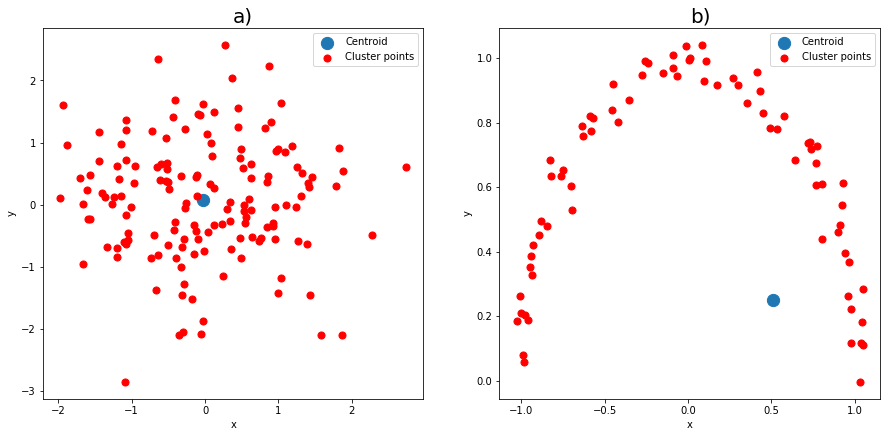
\includegraphics[width=\linewidth]{img/centroids.png}
  \caption{Centroids of a cluster calculated as mean of all points.}
  \label{img:centroids}
\end{figure}

However, if a calculated centroid is not meaningful (see Figure~\ref{img:centroids} b)), a medoid can be selected as an alternative to it.
A medoid is a point that is in the set that minimizes the average distance to all the other points in the set.
It can be thought of as a median of the dataset.
Formally, medoid is defined as:
\begin{equation}
x_{medoid} = \mathrm{argmin}_{y \in \{x_1, x_2, ..., x_n\}} \sum_{i=1}^{n}{d(y, x_i)}\:, \tag{5}
\end{equation}
where $x_1, x_2, ..., x_n$ is a set of $n$ points in a space with a distance function $d$.
In Figure~\ref{img:medoids}, medoids were chosen instead of centroids.
\begin{figure}
  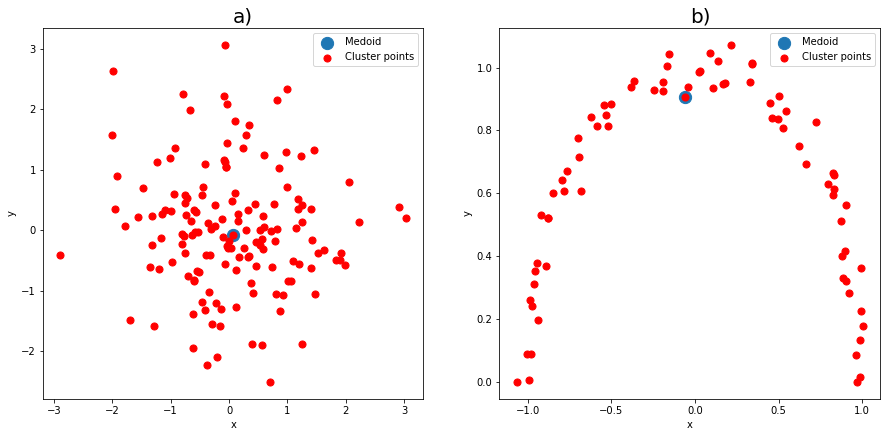
\includegraphics[width=\linewidth]{img/medoids.png}
  \caption{Choice of medoids}
  \label{img:medoids}
\end{figure}

\subsection{Representative Selection in a Topological Space}\label{sec:rep_select_arbitrary}
According to the previous section, the concept of centroid cannot be used to solve the problem of finding a representative in an arbitrary space (i.e., topological space).
Instead, medoids can be selected for datasets in arbitrary spaces.

$K$-Medoids algorithm resembles $K$-means algorithm in breaking the dataset into $K$ groups.
In these groups it finds a medoid that is minimizes the distance to each other point in the group.
$K$-Medoids is most commonly used for representative selection in topological spaces.

There are not many other well-explored methods for solving the problem of finding medoids.
The one that is used in this thesis is explained in \cite{liebman2015representative}.
The main ideas from $K$-means clustering were taken and transformed for usage in a non-metric space with a pair-wise similarity measure.
Instead of stating the $K$ in advance they state a parameter  $ 0 \leq \delta \leq 1$ that serves as a constraint.
Then they separate the cluster into subclusters based on this parameter.
Each of these subclusters is represented by a medoid.
A set of these medoids then serves as a cluster prototype for the whole cluster.
This method is explained in greater detail in the Section~\ref{subsec:delta_medoids}.

\section{Algorithms Relevant for Topological Space}\label{sec:relevant_methods}
Based on the previously explained approaches for finding representatives of clusters in non-metric spaces, the following methods were chosen, tested and compared as a part of this thesis.
\begin{itemize}
    \item Random selection
    \item Greedy Selection
    \item $\delta$-Medoids One-Shot
    \item $\delta$-Medoids
\end{itemize}

\subsection{Random Selection}\label{subsec:random_select}

Random selection algorithm serves as a baseline to measure the improvement as it is the method currently used in Cognitive Targeted Anomaly Detection Framework.
It selects a given number of representatives from the cluster randomly.

In dense clusters, selecting random samples from each cluster leads to undesired noise.
However as experimental results presented in \cite{kopp2018community} in the domain of computer networks, the density of clusters is not significant.
It, of course, depends on each network, but given the best practices in segmentation of networks, the overlaps in clusters are not expected to be great.

\subsection{Greedy Selection}\label{subsec:greedy_select}
The greedy selection algorithm is a straightforward algorithm that selects a random sample from the set as the first representative.
Then it looks for the most different sample in the rest of the dataset.
Once the desired sample is found, the algorithm removes all neighboring samples with at least the similarity of $\delta$ from the set.
Then it looks for other dissimilar samples until the whole set is represented.

The speed of this algorithm depends on the sparsity of the given set.
In the worst case scenario, all points would be selected as representatives while always calculating the distance to each remaining sample in the set. Then it would reach the time complexity of $\mathcal{O}(n^2)$.

\subsection{$\delta$-Medoids}\label{subsec:delta_medoids}
The two following algorithms were first explained in \cite{liebman2015representative}.
They were tested on two different problems that also use clustering in non-metric space - computing distance of two musical segments and comparing trajectories of objects.

$\delta$-Medoids algorithm tries to find a minimal subset of points that are needed to cover the cluster with only one given constraint, that distance of the representatives would be at least $\delta$.
There are two versions of this algorithm.
One-shot version is faster but less precise than the full $\delta$-medoids algorithm.

\subsection{$\delta$-Medoids One-Shot}

The idea behind this algorithm is to go through the dataset looking for representatives that differ at least by the given parameter $\delta$ from each previously selected representatives.
By taking this approach, it can in one iteration over data find the representatives that are certain to differ by $\delta$ from each other.

The pseudocode of this algorithm is shown in Algorithm~\ref{alg:delta_medoids_one_shot}.
It have been optimized for better memory efficiency as opposed to the version in the cited paper.
The main ideas remain the same, only keeping track of clusters that the points are assigned to is removed for this one-shot version.

\begin{algorithm}
    \caption{$\delta$-Medoids One-shot}
    \label{alg:delta_medoids_one_shot}
    \begin{algorithmic}[1]
        \INPUT data $x_0$ ... $x_m$, required distance $\delta$
        \STATE Initialize \textit{representatives} = $\emptyset$
        \FOR{$i = 0$ \textbf{to} $m$}
            \STATE Initialize \textit{dist} = $\infty$
            \FOR{\textit{rep} in \textit{representatives}}
                \IF{$d(x_i, rep) \le dist$}
                    \STATE $dist = d(x_i, rep)$
                \ENDIF
            \ENDFOR
            \IF{$dist > \delta$}
                \STATE add $x_i$ to \textit{representatives}
            \ENDIF
        \ENDFOR
    \end{algorithmic}
\end{algorithm}


The choice of the first representative strongly influences the selection of the medoids to represent the cluster.
In some cases, this one-shot approach could be misleading.

\subsection{$\delta$-Medoids Full}

The full version of the algorithm runs a one-shot algorithm multiple times.
Each time it goes through the dataset it selects a better medoid than before.
If two consecutive passes through the data do not change any medoid, the algorithm stops.
This algorithm is shown in Algorithm~\ref{alg:delta_medoids_full}.
Original algorithm from \cite{liebman2015representative} lacks the routine \textit{ReduceClusters} on line 24.
This routine is introduced in this thesis as an improvement of the algorithm because the original algorithm selected too many representatives.
It is explained in greater detail in the Section~\ref{sec:modified}

This approach is slower than $\delta$-Medoids, as the main routine from one shot algorithm has to be run multiple times.
Experimental results of \cite{liebman2015representative} show that the algorithm converges in very few ($<$10) cycles. \todo{To samozrejme zalezi na volbe datasetu, jak to jednoduse vysvetlit.}
On the other hand, it is able to select better medoids, thus getting rid of the difficult choice of the first representative to select.

\begin{algorithm}
    \caption{$\delta$-Medoids}
    \label{alg:delta_medoids_full}
    \begin{algorithmic}[1]
        \INPUT data $x_0$ ... $x_m$, required distance $\delta$
        \STATE $t = 0$
        \STATE Initialize $representatives_{t_0} = \emptyset$
        \STATE Initialize \textit{clusters} = $\emptyset$
        \DO
            \STATE $t = t + 1$
            \FOR{$i = 0$ \textbf{to} $m$}
                \STATE Initialize \textit{dist} = $\infty$
                \STATE Initialize \textit{representative = null}
                \FOR{\textit{rep} in \textit{representatives}}
                    \IF{$d(x_i, rep) \le dist$}
                        \STATE \textit{representative = rep}
                        \STATE $dist = d(x_i, rep)$
                    \ENDIF
                \ENDFOR
                \IF{$dist \le \delta$}
                    \STATE add $x_i$ to $cluster_{representative}$
                \ELSE
                    \STATE \textit{representative = $x_i$}
                    \STATE Initialize $cluster_{representative} = \emptyset$
                    \STATE add $x_i$ to $cluster_{representative}$
                    \STATE add $cluster_{representative}$ to \textit{clusters}
                \ENDIF
            \ENDFOR
            \STATE Call \textbf{\textit{ReduceClusters}}
            \STATE Initialize $representatives_t = \emptyset$
            \FOR{\textit{cluster} in \textit{clusters}}
                \STATE $representative = \textrm{argmin}_{s \in cluster} (\sum\limits_{x \in cluster}{d(x,s) : d(x,s) \le \delta)}$
                \STATE add \textit{representative} to $representatives_t$
            \ENDFOR
        \DOWHILE{$representatives_t = representatives_{t-1}$}
    \end{algorithmic}
\end{algorithm}

\subsection{$\delta$-Medoids Modified}
\label{sec:modified}

The algorithm $\delta$-Medoids Full does not have any restriction for the number of representatives it selects for each cluster.
Results in Chapter~\ref{ch:experiments} show that the full algorithm can select up to a third of a big complex cluster which does not satisfy the Criterion 1 from Section~\ref{sec:def_rep_selection} properly.
To reduce the number of representatives a subroutine \textit{ReduceClusters} was introduced as a modification to the original algorithm.
The subroutine is shown \textit{ReduceClusters} shown in Algorithm~\ref{alg:reduce}.

The basic idea behind this modification is to get rid of representatives that cover a small portion of the whole dataset by either merging them with similar representatives or dropping them entirely.
If a representative does not cover at least 1\% of the cluster, the routine tries to add it to the coverage of the representative that is the most similar.
If no such similar representative exists, it is considered noise and the representative is dropped from the cluster.

\begin{algorithm}
    \caption{ReduceClusters}
    \label{alg:reduce}
    \begin{algorithmic}[1]
        \INPUT $m$ subclusters $X$ = $x_i, ..., x_m$; their representatives $R = r_0, ..., r_m$; whole cluster size$s$; constant $\kappa$
        \STATE $threshold = 0.01s$
        \STATE Initiate $i = 0$
        \IF{$|X| > \kappa$}
            \WHILE{$i < m$}
                \IF{$|x_i| \le threshold$}
                    \STATE $j$ = index the most similar representative from $R$
                    \IF{no such $j$ exists}
                        \STATE Drop $x_i$ from $X$
                    \ELSE
                        \STATE Merge $x_i$ and $x_j$.
                    \ENDIF
                    \STATE Drop $r_i$ from $R$
                \ENDIF
            \ENDWHILE
        \ENDIF
    \end{algorithmic}
\end{algorithm}

Figure~\ref{img:complexity} shows that $\delta$-Medoids Modified is a bit faster than the version full version.
This combined with the fact that it selects lower number of representatives shows that the modification improved its performance for this thesis's use case.

\begin{figure}
  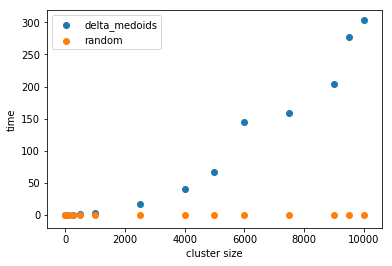
\includegraphics[width=\linewidth]{img/complexity.png}
  \caption{Comparing run times of $\delta$-Medoids and Random Selection}
  \label{img:complexity}
\end{figure}

%========================================CHAPTER==================================

\chapter{Datasets}\label{ch:datasets}

The task of cluster representation in non-metric spaces generally is not necessarily connected only to the security field.
Before moving to a dataset collected from a real network, the selected algorithms were first tested on artificially created datasets and well-labeled datasets found in the literature.

Below, the datasets used in this thesis are presented.
Three types of datasets were used: artificially created, image recognition and real network security dataset.
Each section corresponds to one of the listed dataset types.

\section{Datasets Created for this Work}

These datasets were created to test the specific properties of tested methods.
They were made by using the Scikit-Learn library for Python 3 \cite{scikit-learn}.
The datasets created are the following:
\begin{itemize}
    \item Blobs 3D
    \item Overlap
    \item Circles 3D
    \item Moons
\end{itemize}
All of these datasets are in a metric space of two or three dimensions.
They can be easily visualized on graphs and show some of the specific properties of implemented algorithms.
\begin{figure}
  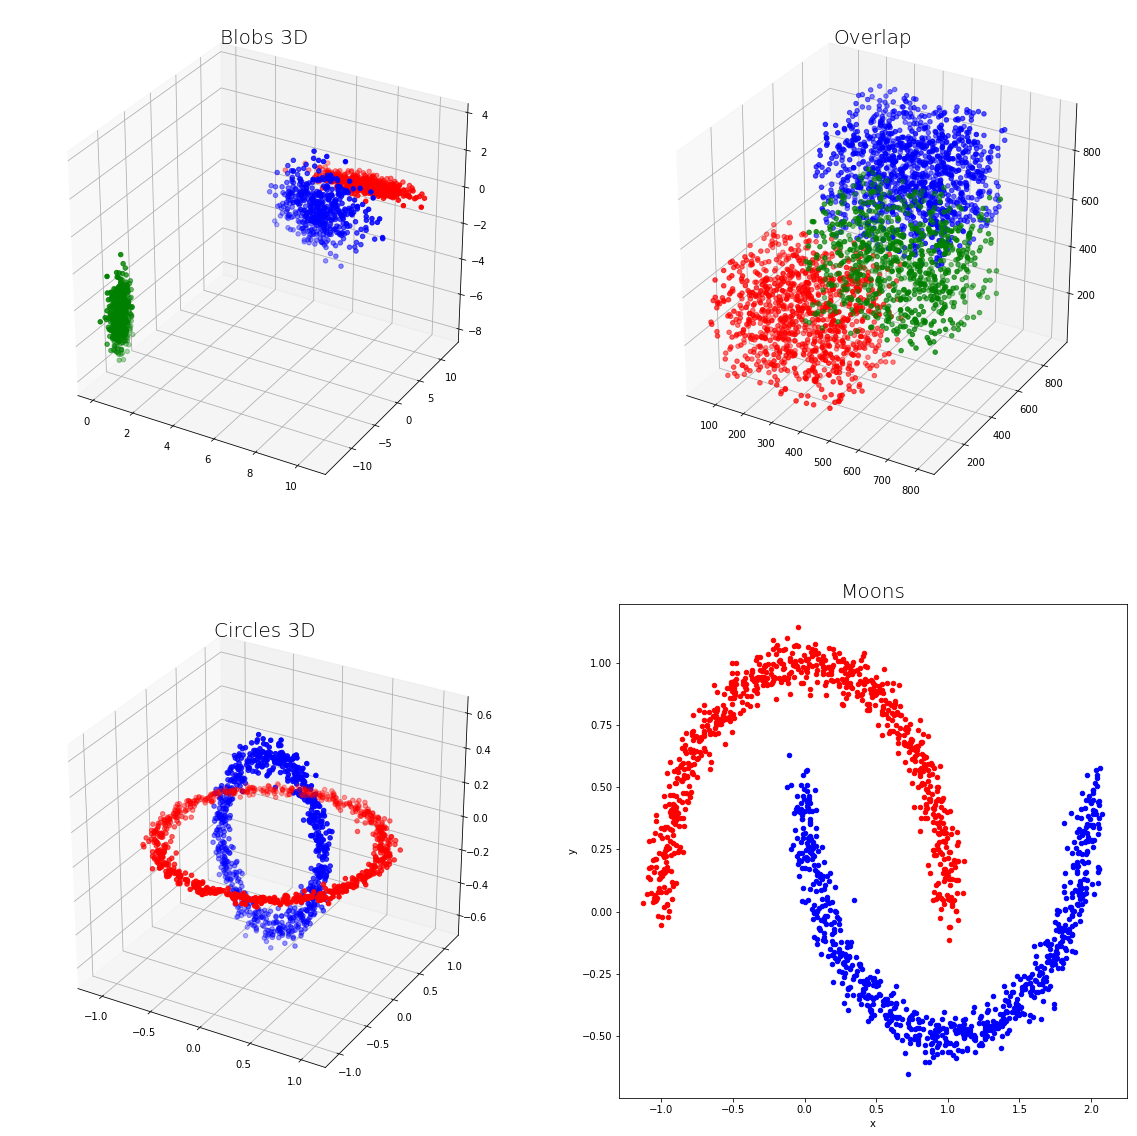
\includegraphics[width=\linewidth]{img/datasets.png}
  \caption{Graphs of all datasets}
  \label{img:datasets}
\end{figure}

The Blobs 3D dataset consists of three clusters that are scattered randomly around a center point.
This dataset was selected to test what samples will be selected by methods explained in Chapter~\ref{ch:theory} in clusters that can be easily represented by a centroid.
The Overlap dataset consists of 3 clusters in shapes of blocks.
These blocks overlap partly to test how selected algorithms cope with overlapping clusters.
Circles 3D and Moons are one of the hardest datasets to represent even by methods that are designed specifically for the metric space.
These two datasets were chosen to test the resistance to noise in selecting representatives.
All of these datasets are shown in Figure~\ref{img:datasets}.

\section{Image Recognition Datasets}
One of the best-documented application domains for clustering is image recognition.
Therefore, two datasets from this area were chosen for measuring the precision of each method.
The first one is a labeled dataset of features collected from handwritten digits.
The other one consists of annotated black and white pictures of clothing, shoes, and handbags.

The Pen-Based Recognition of Handwritten Digits Data Set \cite{dua1998pendigit} consists of 10922 samples.
A sample represents 16 features collected from a handwritten digit.
For each digit, there is a little more than a thousand samples.
Features represent coordinate information about the digits as they were written on a $500\times500$ pixel frame.
This dataset is split to train dataset (70\%) and test dataset (30\%).

The MNIST Fashion dataset \cite{xiao2017fashion} consists of a training set of 60,000 samples and 10,000 test samples.
A sample from this dataset is a grayscale image of a piece of clothing, a shoe or a handbag.
Each sample belongs to one of 10 classes.
This problem is more complicated than handwritten digits from the previous dataset.
It is a current benchmark dataset for classification problems.
The MNIST Fashion dataset was introduced quite recently, in 2017.

\section{Network Security Dataset}\label{sec:real-data}
Real network traffic captured from a company with approximately 20 thousand employees.
The capture is from more than 24 hours of a working day and consists of 33.5  million flows.
Hosts that appeared in that capture were clustered using the method explained in Section~\ref{sec:cluster_topo}.
There are 16 clusters with sizes ranging from less than a hundred to several thousand.
These clusters with all hosts labeled were used as real network dataset in this thesis.
Labels provided for this dataset are the output of community-based clustering in Cognitive Targeted Anomaly Detection Framework.
Similarity threshold used for the clustering was 0.8.

Each sample represents one device on the network.
For such a big network the behaviors of devices are very diverse.
This leads to heterogeneous clusters with behavior that changes over time.
Only a pair-wise similarity between each host pair exists.
Representation of cluster created is a complex problem, suitable for testing the properties of algorithms selected in this thesis.
\todo{expand this if there is time}

%========================================CHAPTER==================================

\chapter{Experiments}\label{ch:experiments}

In this chapter, all performed experiments are described.
Each section represents one experiment with its motivation, experimental setup and results.

All experiments were made in Jupyter Notebook technology using Python 3.7 kernel.
For loading data from files and storing them in memory the Pandas library version 0.23.4 was used \cite{mckinney2010data}.

There are two main criteria for evaluating the result of each experiment.
One is the number of selected samples.
The other one is the coverage provided by these representatives.
A table with these two measures is presented for each experiment.

For testing the ability to assign new samples to its corresponding cluster a part of each dataset was separated as test data.
The algorithms $K$-Nearest Neighbors with $K=1$ was then used to classify the test data based on the cluster prototypes created by selected algorithms.
For each dataset, a confusion matrix was created to visualize the results of the classification test.

\section{Visualizable datasets}\label{sec:exp1}

The first experiment was run on the visualizable datasets created explicitly for this thesis.
Seeing clustering results on visualizable datasets provides insight into algorithms performance.

The methods that were explained in Section~\ref{sec:relevant_methods} are usable on metric space with a distance measure as metric space is a special case of a topological space for which they are desiged.
Using them on visualizable benchmark datasets designed to address specific problems helped to determine their properties such as how many representatives each algorithm selects and how well does the representatives work in classification in newly added samples.

\subsection{Experimental Setup}
Datasets used for this experiment were:
\begin{itemize}
    \item Blobs 3D
    \item Overlap
    \item Moons
    \item Circles 3D
\end{itemize}

All five algorithms were run.
The $\delta$ was estimated as 5\% quantile of distances from one random point in the data to all of the others.
This choice was made because the desired number of samples selected is around 20.
The similarity measure used in these datasets was Euclidean distance.

This experiment was performed in five runs using cross-validation.
Each dataset was split into five 20\% parts.
In each run, four parts were combined to form the training data, and the remaining part was used to simulate newly added samples to be classified to their corresponding cluster.

\subsection{Results}

The results for each dataset are listed below.
A table with the number of representatives selected from each cluster is presented as well as confusion matrix with correct and incorrect classifications of each test sample.
\medskip

\textbf{Blobs 3D}
\begin{table}[H]
\resizebox{\textwidth}{!}{
\begin{tabular}{l|llllll}
\hline
 \textbf{Cluster} & \specialcell{\textbf{Training}\\ \textbf{Samples}} & \specialcell{\textbf{Greedy}\\ \textbf{Selection}} & \specialcell{\textbf{$\delta$-Medoids}\\ \textbf{One-Shot}} & \specialcell{\textbf{$\delta$-Medoids}\\ \textbf{Full}} & \specialcell{\textbf{$\delta$-Medoids}\\ \textbf{Modified}} & \specialcell{\textbf{Random}\\ \textbf{Selection}} \\ \hline
A & 400 & 21 (100)& 23 (100)& 25 (100)& 16 (96.75)& 16 (86.25)\\
B & 400 & 17 (100)& 20 (100)& 23 (100)& 20 (99)& 20 (92.75)\\
C & 400 & 19 (100)& 20 (100)& 22 (100)& 20 (99.25)& 20 (92)\\ \hline
\end{tabular}}
\caption{Number of selected representatives with coverate in percent for the Blobs 3D dataset}
\end{table}

\noindent For the Blobs dataset, which is an easy representation problem, all algorithms were able to cover the dataset almost perfectly.
Lower coverage for Random Selection can be seen but the density and distribution of samples still makes it cover most of the cluster.
The lower coverage of $\delta$-Medoids Modified falls into a 5\% ratio, which rules out the extreme borders of the cluster.
This is very good as the algorithm is not expected to cover samples that are too distant from the rest of the custer.

The number of representatives selected is aproximately 20, that highly corresponds with the choice of $\delta$.
This does is not a problem as the number is still relatively small (less than 10\% of the dataset).
Also, in Cognitive Targeted Anomaly Detection Framework, clusters do dynamically change, and a around 20 representatives is requested to keep track of the cluster over time.

The confusion matrix of classification test can be seen in Figure~\ref{img:exp1_blobs}.

\begin{figure}[H]
   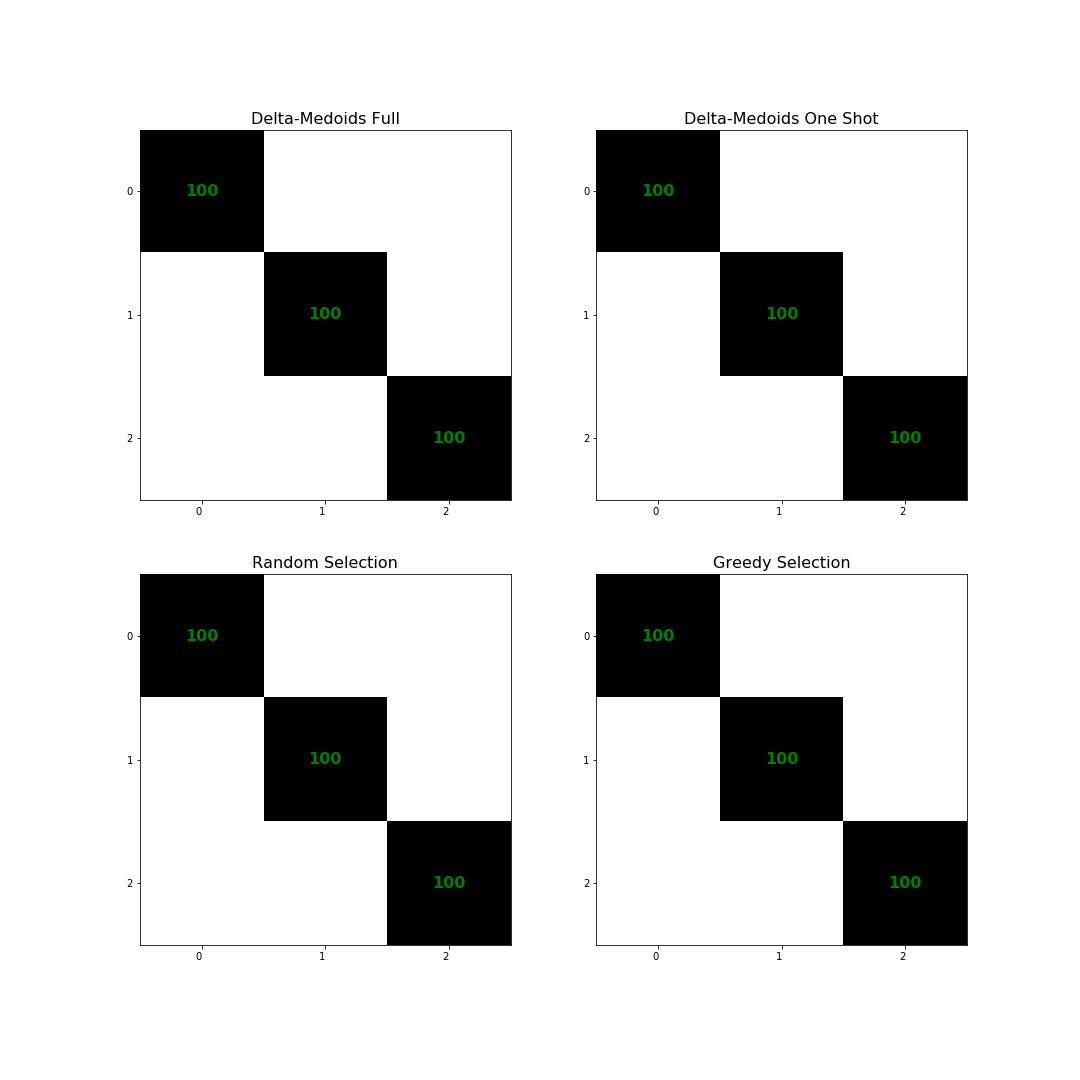
\includegraphics[width=\linewidth]{img/exp1_blobs.png}
  \caption{Confusion matrices for Blobs 3D dataset}
  \label{img:exp1_blobs}
\end{figure}
\medskip

\textbf{Overlap}

\begin{table}[H]
\resizebox{\textwidth}{!}{
\begin{tabular}{l|llllll}
\hline
 \textbf{Cluster} & \specialcell{\textbf{Training}\\ \textbf{Samples}} & \specialcell{\textbf{Greedy}\\ \textbf{Selection}} & \specialcell{\textbf{$\delta$-Medoids}\\ \textbf{One-Shot}} & \specialcell{\textbf{$\delta$-Medoids}\\ \textbf{Full}} & \specialcell{\textbf{$\delta$-Medoids}\\ \textbf{Modified}} & \specialcell{\textbf{Random}\\ \textbf{Selection}} \\ \hline
A & 800 & 25 (100)& 23 (100)& 23 (100)& 23 (99.75)& 23 (87.88)\\
B & 960 & 26 (100)& 21 (100)& 23 (100)& 21 (100)& 21 (81.15)\\
C & 640 & 22 (100)& 24 (100)& 24 (100)& 24 (99.84)& 24 (88.6)\\ \hline
\end{tabular}}
\caption{Number of selected representatives with coverate in percent for the Overlap dataset}
\end{table}
\noindent In the Overlap dataset, the average fit of the data remains similar to the Blobs 3D dataset as it is calculated for each cluster separately.
Therefore, the number of representatives selected remains determined only by the choice of $\delta$.

The results of the classification test show, classifying border samples from overlapping clusters is not a simple task.
Confusion matrices present a slightly better results with the representatives selected by $\delta$-Medoids modified.
However the number of misclassified samples for each dataset is not significant when compared to the number of samples in the cluster.
The confusion matrix can be seen in Figure~\ref{img:exp1_overlap}.

\begin{figure}[H]
   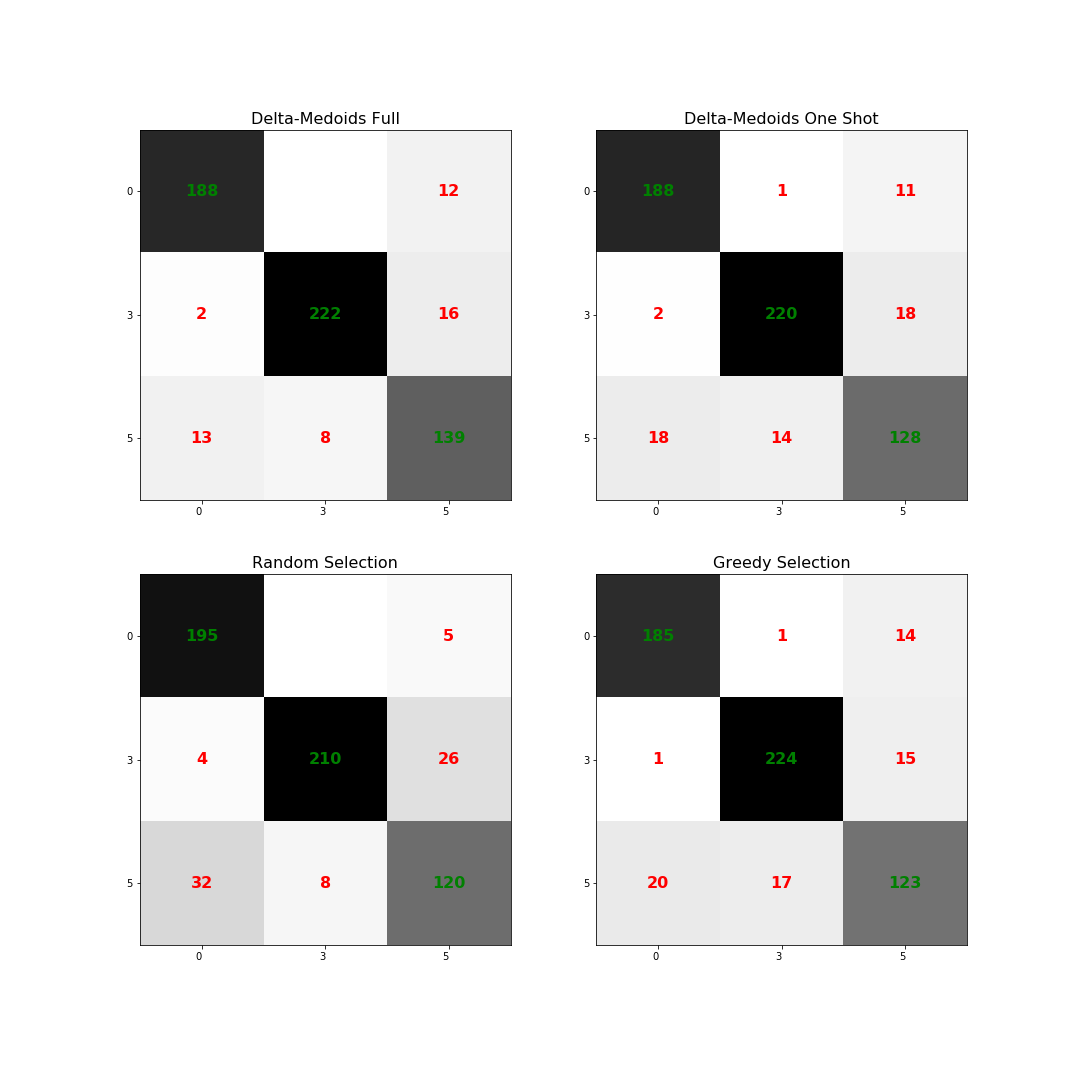
\includegraphics[width=\linewidth]{img/exp1_overlap.png}
  \caption{Confusion matrices for Overlap dataset}
  \label{img:exp1_overlap}
\end{figure}
\medskip
\textbf{Moons and Circles 3D}

\begin{table}[H]
\resizebox{\textwidth}{!}{
\begin{tabular}{l|llllll}
\hline
 \textbf{Cluster} & \specialcell{\textbf{Training}\\ \textbf{Samples}} & \specialcell{\textbf{Greedy}\\ \textbf{Selection}} & \specialcell{\textbf{$\delta$-Medoids}\\ \textbf{One-Shot}} & \specialcell{\textbf{$\delta$-Medoids}\\ \textbf{Full}} & \specialcell{\textbf{$\delta$-Medoids}\\ \textbf{Modified}} & \specialcell{\textbf{Random}\\ \textbf{Selection}} \\ \hline
A & 600 & 22 (100)& 21 (100)& 22 (100)& 21 (100)& 21 (88.67)\\
B & 600 & 21 (100)& 24 (100)& 25 (100)& 24 (100)& 24 (67)\\ \hline
\end{tabular}}
\caption{Number of selected representatives with coverate in percent for the Moons dataset}
\end{table}

\begin{table}[H]
\resizebox{\textwidth}{!}{
\begin{tabular}{l|llllll}
\hline
 \textbf{Cluster} & \specialcell{\textbf{Training}\\ \textbf{Samples}} & \specialcell{\textbf{Greedy}\\ \textbf{Selection}} & \specialcell{\textbf{$\delta$-Medoids}\\ \textbf{One-Shot}} & \specialcell{\textbf{$\delta$-Medoids}\\ \textbf{Full}} & \specialcell{\textbf{$\delta$-Medoids}\\ \textbf{Modified}} & \specialcell{\textbf{Random}\\ \textbf{Selection}} \\ \hline
A & 600 & 15 (100)& 13 (100)& 13 (100)& 13 (100)& 13 (87.5)\\
B & 600 & 6  (100)& 8  (100)& 8  (100)& 8  (99.83)&  8 (83.5)\\ \hline
\end{tabular}}
\caption{Number of selected representatives with coverate in percent for the Circles 3D dataset}
\end{table}

\noindent Selecting representatives both Moons and Circles 3D datasets is harder problem than for the compact clusters in Blobs 3D and Ovverlap datasets.
Clusters in the Moons dataset are not easily represented by one centroid.
The results show that medoid selection is a good option for representing this type of clusters.
Each method, excluding Random Selection was able to cover the whole cluster.
Randomly selected representatives suffer from the uneven distribution of samples in the space, thus covering a lower portion of the cluster.
On these two datasets, the Random Selection algorithm performs worse as can be seen in the corresponding confusion metrices.
The confusion matrix for the Moons dataset can be seen in Figure~\ref{img:exp1_moons}, for the Circles 3D dataset in Figure~\ref{img:exp1_circles}


\begin{figure}[h]
   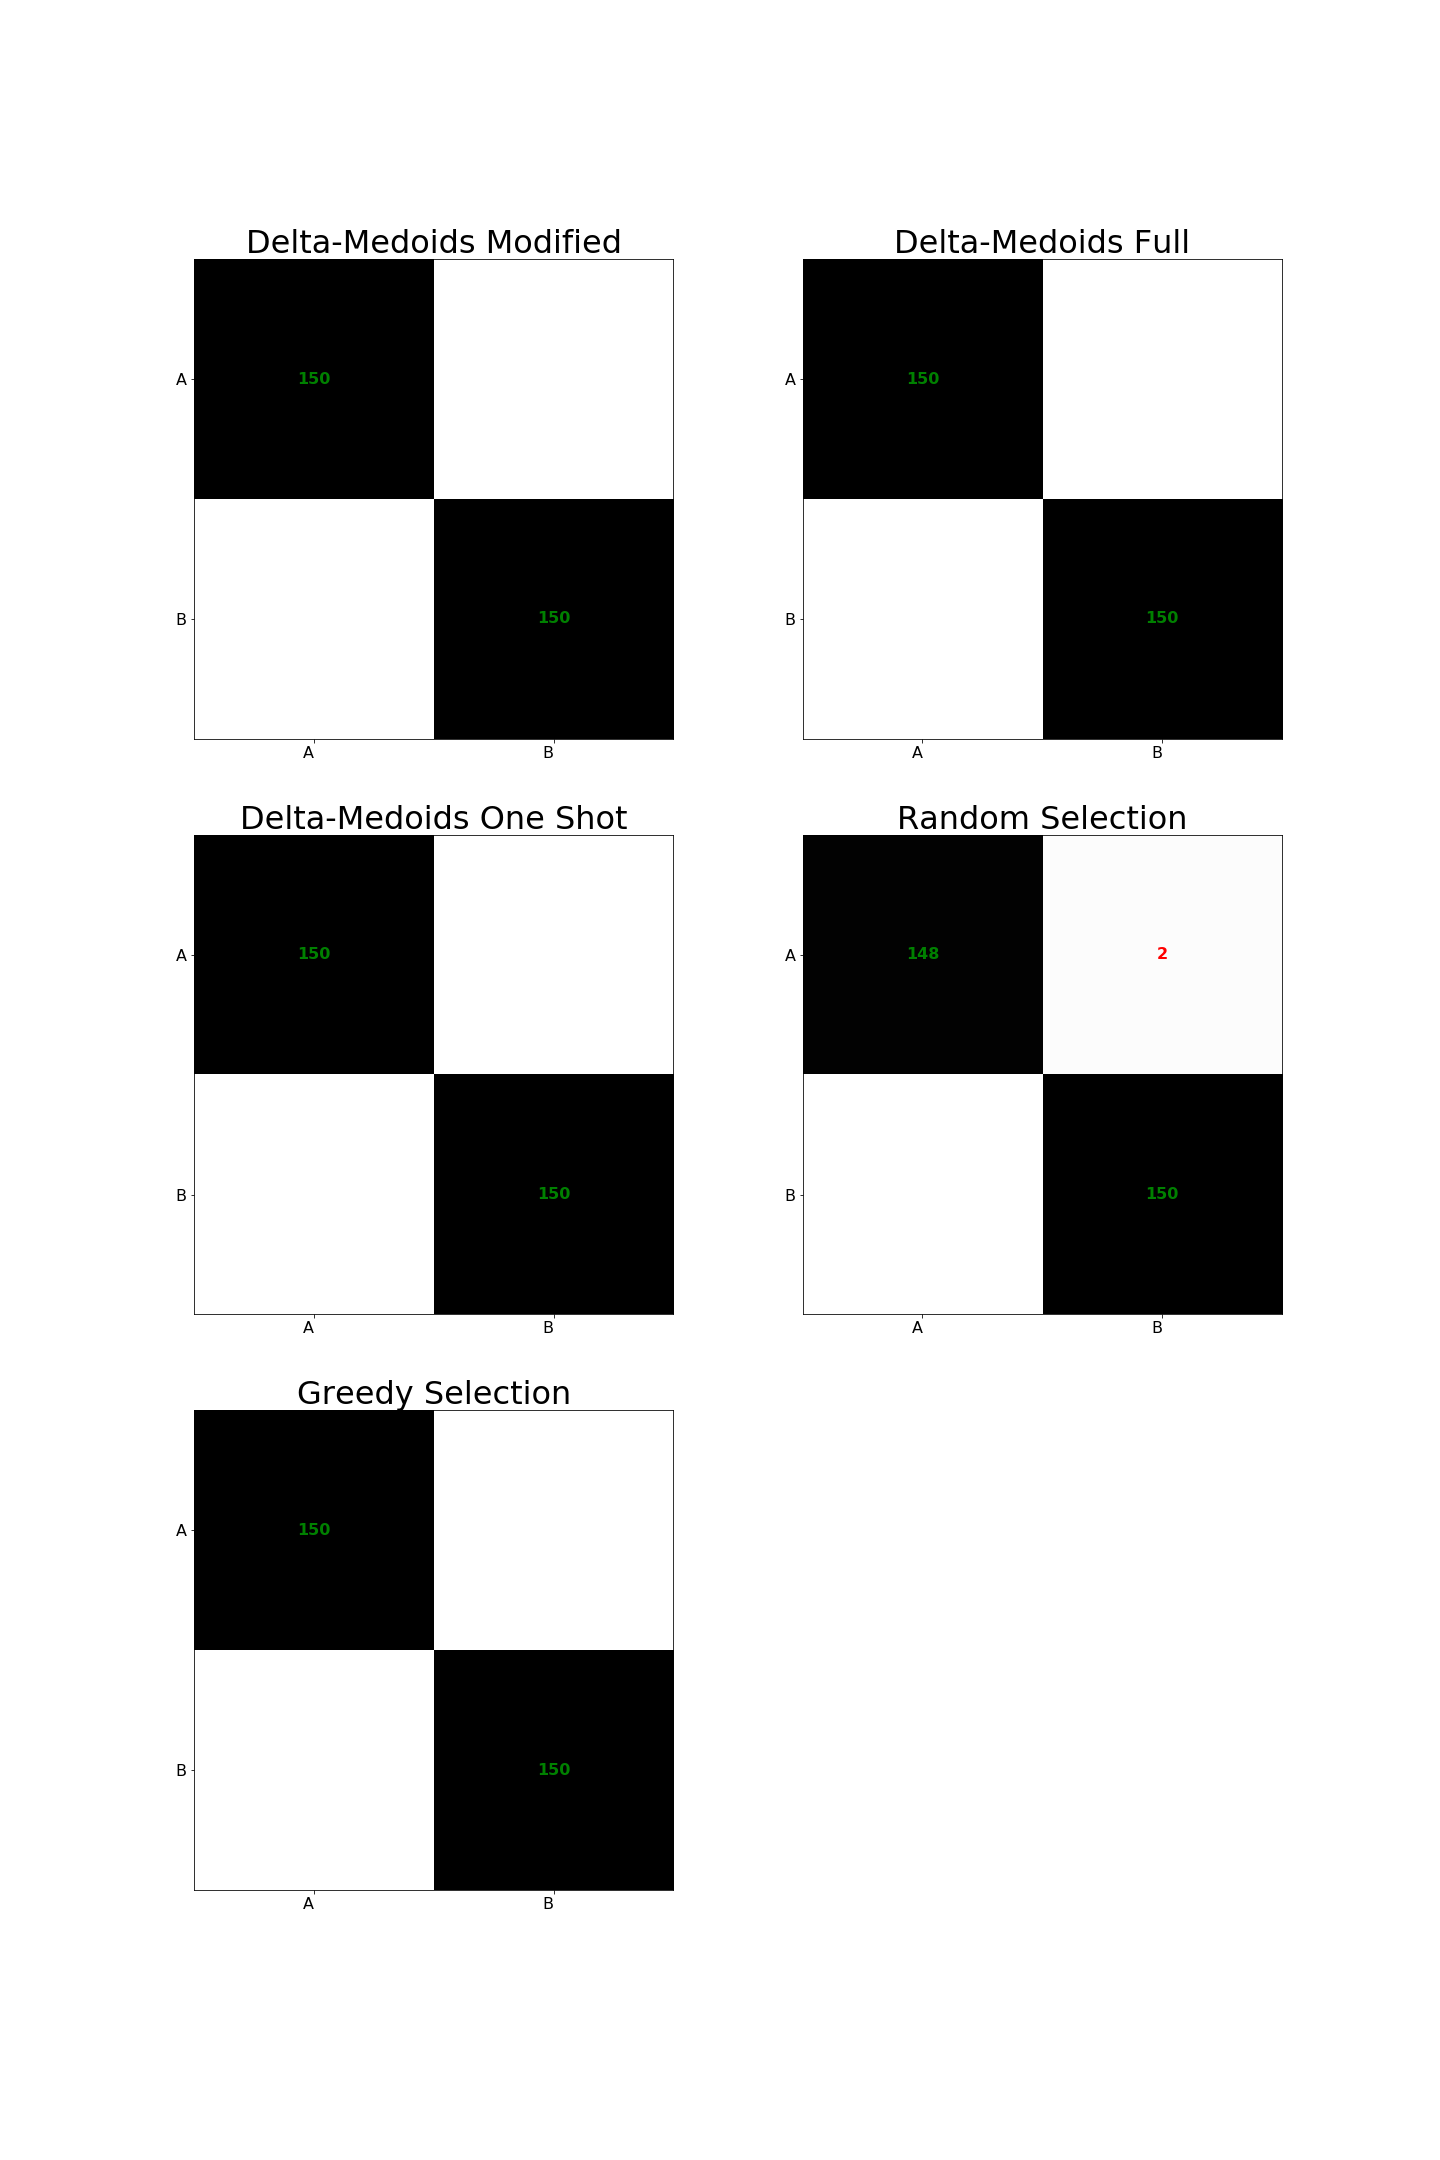
\includegraphics[width=\linewidth]{img/exp1_moons.png}
  \caption{Confusion matrices for Moons dataset}
  \label{img:exp1_moons}
\end{figure}

\begin{figure}[h]
   \includegraphics[width=\linewidth]{img/exp1_circles.png}
  \caption{Confusion matrices for Circles 3D dataset}
  \label{img:exp1_circles}
\end{figure}

From the results listed the difference between $\delta$-Medoids Full and Modified are not easily distinguishable.
The difference between these two algorithms can be seen in Figure~\ref{img:difference_modified}.
The full version of the algorithm tends to select the border samples of a dataset as representatives.
In these datasets, the results do not show this because they are relatively dense and have a normal distribution.
On sparser datasets, this leads to a high number of representatives selected, while many of them are not relevant. \todo{make a dataset for this or delete it, time reasons ;( }

\begin{figure}[h]
   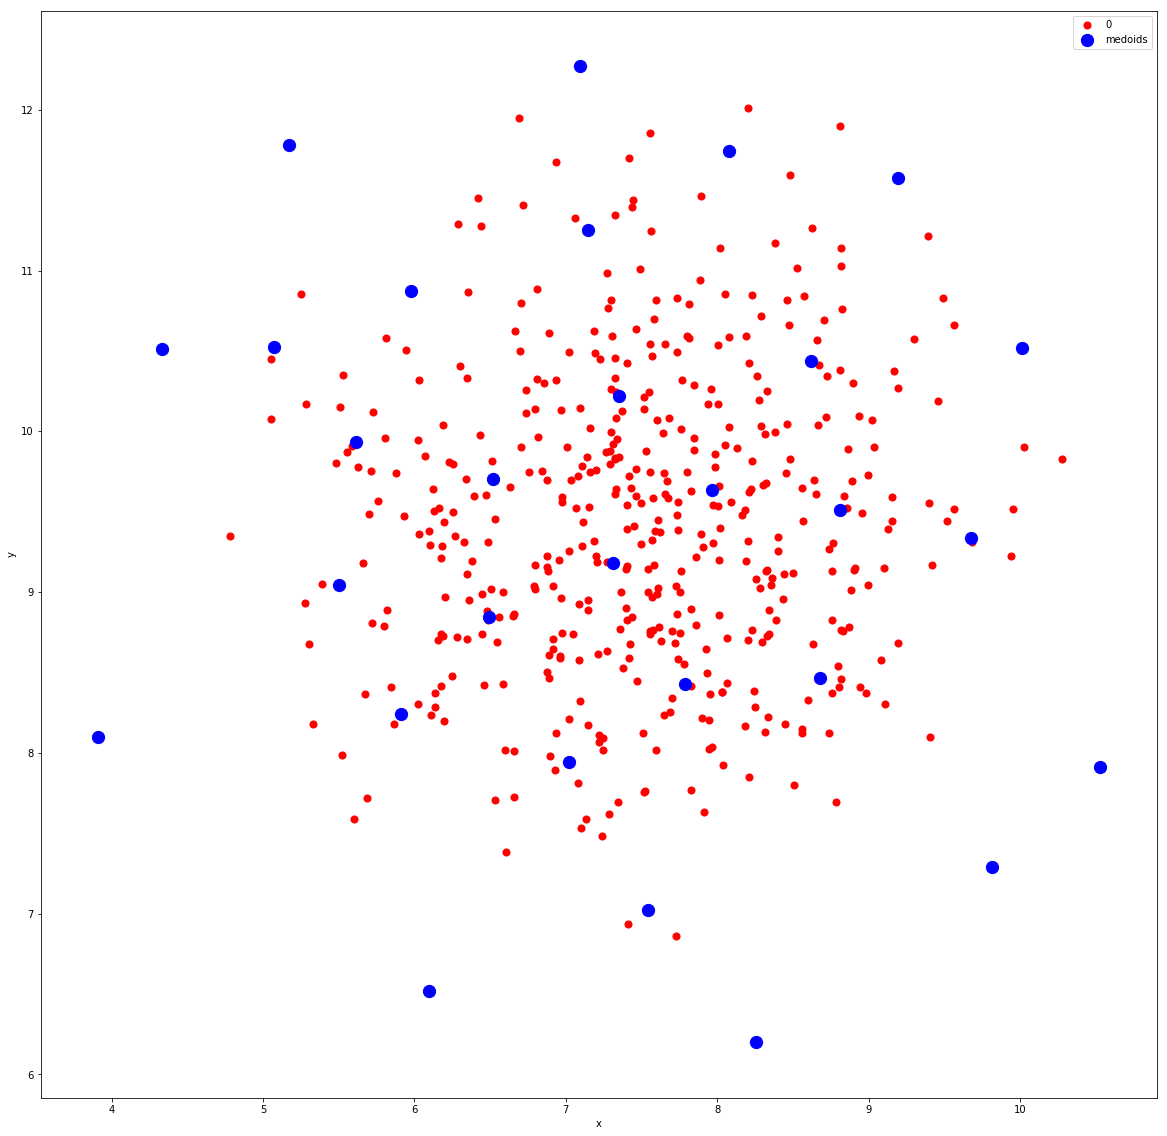
\includegraphics[width=\linewidth]{img/delta_medoids_select.png}
  \caption{Difference between $\delta$-Medoids Full and Modified}
  \label{img:difference_modified}
\end{figure}

\newpage

\section{Test on Image Recognition Datasets}\label{sec:exp3}

The motivation for this experiment was to test the algorithm results on well-explored and well-annotated datasets commonly used as a benchmark for clustering.

\subsection{Experimental Setup}
Datasets used for this experiment were:
\begin{itemize}
    \item Pendigits
    \item MNIST Fashion
\end{itemize}

In this and the following experiments, the $\delta$-Medoids Full algorithm was not used, and only the Modified algorithm was tested.
The $\delta$ was estimated as 5\% quantile of distances from one random point in the data to all of the others.
The similarity measure used in these datasets was Euclidean distance.

\subsection{Results}

The results for different methods are listed below.

\textbf{Pendigits}
\begin{table}[H]
\resizebox{\textwidth}{!}{
\begin{tabular}{l|lllll}
\hline
 \textbf{Cluster} & \specialcell{\textbf{All}\\ \textbf{Samples}} & \specialcell{\textbf{Greedy}\\ \textbf{Selection}} & \specialcell{\textbf{$\delta$-Medoids}\\ \textbf{One-Shot}} & \specialcell{\textbf{$\delta$-Medoids}\\ \textbf{Modified}} & \specialcell{\textbf{Random}\\ \textbf{Selection}} \\ \hline
0 & 780 & 33 (100)& 33 (100)& 33 (100)& 33 (93.46)\\
1 & 779 & 33 (100)& 41 (100)& 41 (100)& 41 (94.48)\\
2 & 780 & 17 (100)& 15 (100)& 15 (100)& 15 (95.71)\\
3 & 719 & 12 (100)& 9  (100)& 9  (100)& 9  (94.64)\\
4 & 780 & 25 (100)& 24 (100)& 24 (100)& 24 (93.59)\\
5 & 720 & 25 (100)& 27 (100)& 27 (100)& 27 (93.89)\\
6 & 720 & 16 (100)& 16 (100)& 16 (100)& 16 (97.3)\\
7 & 778 & 22 (100)& 20 (100)& 20 (100)& 20 (94.24)\\
8 & 719 & 75 (100)& 77 (100)& 15 (100)& 15 (91.24)\\
9 & 719 & 50 (100)& 52 (100)& 13 (100)& 13 (92.65)\\ \hline
\end{tabular}}
\caption{Number of selected representatives with coverate in percent for the Pendigit dataset}
\end{table}
\noindent The confusion matrix can be seen in Figure~\ref{img:exp3_pendigits}
\medskip

\begin{figure}[t]
   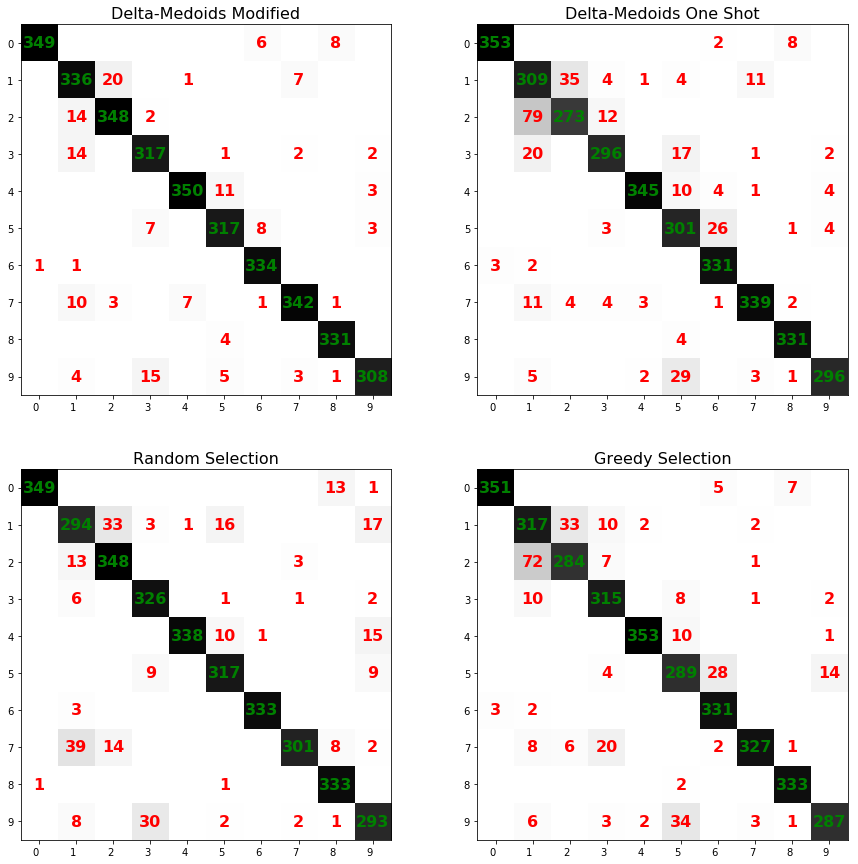
\includegraphics[width=\linewidth]{img/exp3_pendigits.png}
  \caption{Confusion matrices for Pendigits dataset}
  \label{img:exp3_pendigits}
\end{figure}

\textbf{MNIST Fashion}

In the experiment for this dataset, the Greedy Selection algorithm was omitted as the experiments would take too long on clusters that contain 6000 samples.
Previous experiments show that the $\delta$-Medoids algorithm chooses a similar amount of representatives while getting better coverage.

\begin{table}[H]
\resizebox{\textwidth}{!}{
\begin{tabular}{l|lllll}
\hline
 \textbf{Cluster} & \specialcell{\textbf{All}\\ \textbf{Samples}} & \specialcell{\textbf{$\delta$-Medoids}\\ \textbf{One-Shot}} & \specialcell{\textbf{$\delta$-Medoids}\\ \textbf{Modified}} & \specialcell{\textbf{Random}\\ \textbf{Selection}} \\ \hline
0 & 6000 & 859  & 23 & 23 \\
1 & 6000 & 176  & 16 & 16 \\
2 & 6000 & 845  & 20 & 20 \\
3 & 6000 & 616  & 22 & 22 \\
4 & 6000 & 630  & 25 & 25 \\
5 & 6000 & 1622 & 14 & 14 \\
6 & 6000 & 1181 & 18 & 18 \\
7 & 6000 & 266  & 19 & 19 \\
8 & 6000 & 1971 & 16 & 16 \\
9 & 6000 & 686  & 28 & 28 \\ \hline
\end{tabular}}
\caption{Number of selected representatives with coverate in percent for the MNIST Fashion dataset}
\end{table}
\noindent The confusion matrix can be seen in Figure~\ref{img:exp4}
\medskip

\begin{figure}[t]
   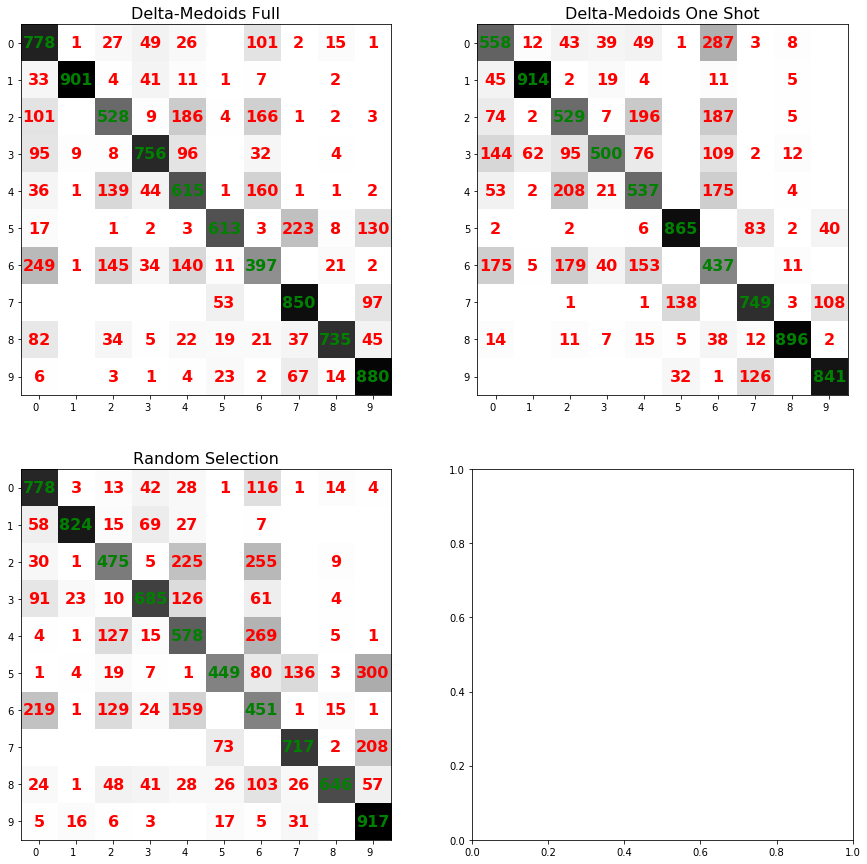
\includegraphics[width=\linewidth]{img/exp3_mnist_fashion.png}
  \caption{Confusion matrices for MNIST Fashion dataset}
  \label{img:exp4}
\end{figure}

\subsection{Conclusion for Image Recognition Datasets}
Using algorithms on real datasets shows more significant differences between results in algorithms.
Especially the difference in numbers of representatives chosen with $\delta$-Medoids Modified while still performing the best in classification test.
The $\delta$-Medoids Modified chooses the lowest number of representatives while getting the best results.
As can be seen in the results for the Pendigits dataset, the Greedy Selection and $\delta$-Medoids One-Shot select similar number of representatives and their results are also very similar.
This is interesting as the complexity of these algorithms differs a lot, Greedy Selection being much slower with $\mathcal{O}(n^2)$.

\section{Network Security Data}\label{sec:exp4}

This experiment tests the functionality of selected methods as if they were plugged into the toolchain of Cognitive Targeted Anomaly Detection described in Section~\ref{sec:ctadf}.
The data for it was collected from the framework, and the experiment was done separately on a different machine.

\subsection{Experimental Setup}
Clustered hosts from a real network were used for this experiment.
This dataset is explained in greater detail in Section~\ref{sec:real-data}.
From this dataset traffic for 24 hours was used for training the model.
Data from the following 4 hours was used for testing the representatives selected.
The similarity measure from Section~\ref{sec:ctadf} was used.

Three algorithms were run, $\delta$-Medoids Full and Greedy Selection were omitted for reasons listed in the previous section.
The $\delta$ was set to 0.8 as was the threshold used in community-based clustering for their creation.

\subsection{Results}

The results for different methods are listed below.

\begin{table}[H]
\resizebox{\textwidth}{!}{
\begin{tabular}{l|lllll}
\hline
 \textbf{Cluster} & \specialcell{\textbf{All}\\ \textbf{Samples}} & \specialcell{\textbf{$\delta$-Medoids}\\ \textbf{One-Shot}} & \specialcell{\textbf{$\delta$-Medoids}\\ \textbf{Modified}} & \specialcell{\textbf{Random}\\ \textbf{Selection}} \\ \hline
A & 72   & 7    & 7  & 7  \\
B & 127  & 23   & 27 & 27 \\
C & 2263 & 1480 & 46 & 46 \\
D & 124  & 76   & 17 & 17 \\
E & 89   & 68   & 16 & 16 \\
F & 54   & 38   & 38 & 38 \\
G & 87   & 41   & 42 & 42 \\
H & 1149 & 503  & 34 & 34 \\
I & 60   & 53   & 12 & 12 \\
J & 77   & 73   & 14 & 14 \\
K & 2692 & 912  & 25 & 25 \\
L & 137  & 109  & 22 & 22 \\
M & 53   & 35   & 35 & 35 \\
N & 259  & 15   & 16 & 16 \\
O & 76   & 58   & 13 & 13 \\
P & 76   & 76   & 7  & 7  \\ \hline
\end{tabular}}
\caption{Number of selected representatives with coverate in percent for the real network data}
\end{table}
\noindent The confusion matrix can be seen in Figure~\ref{img:exp4}
$\delta$-Medoids One Shot algorithm shows better results in classification as the number of representatives selected by this algorithm is significantly higher containing on average 30\% of each cluster.

\begin{figure}[t]
   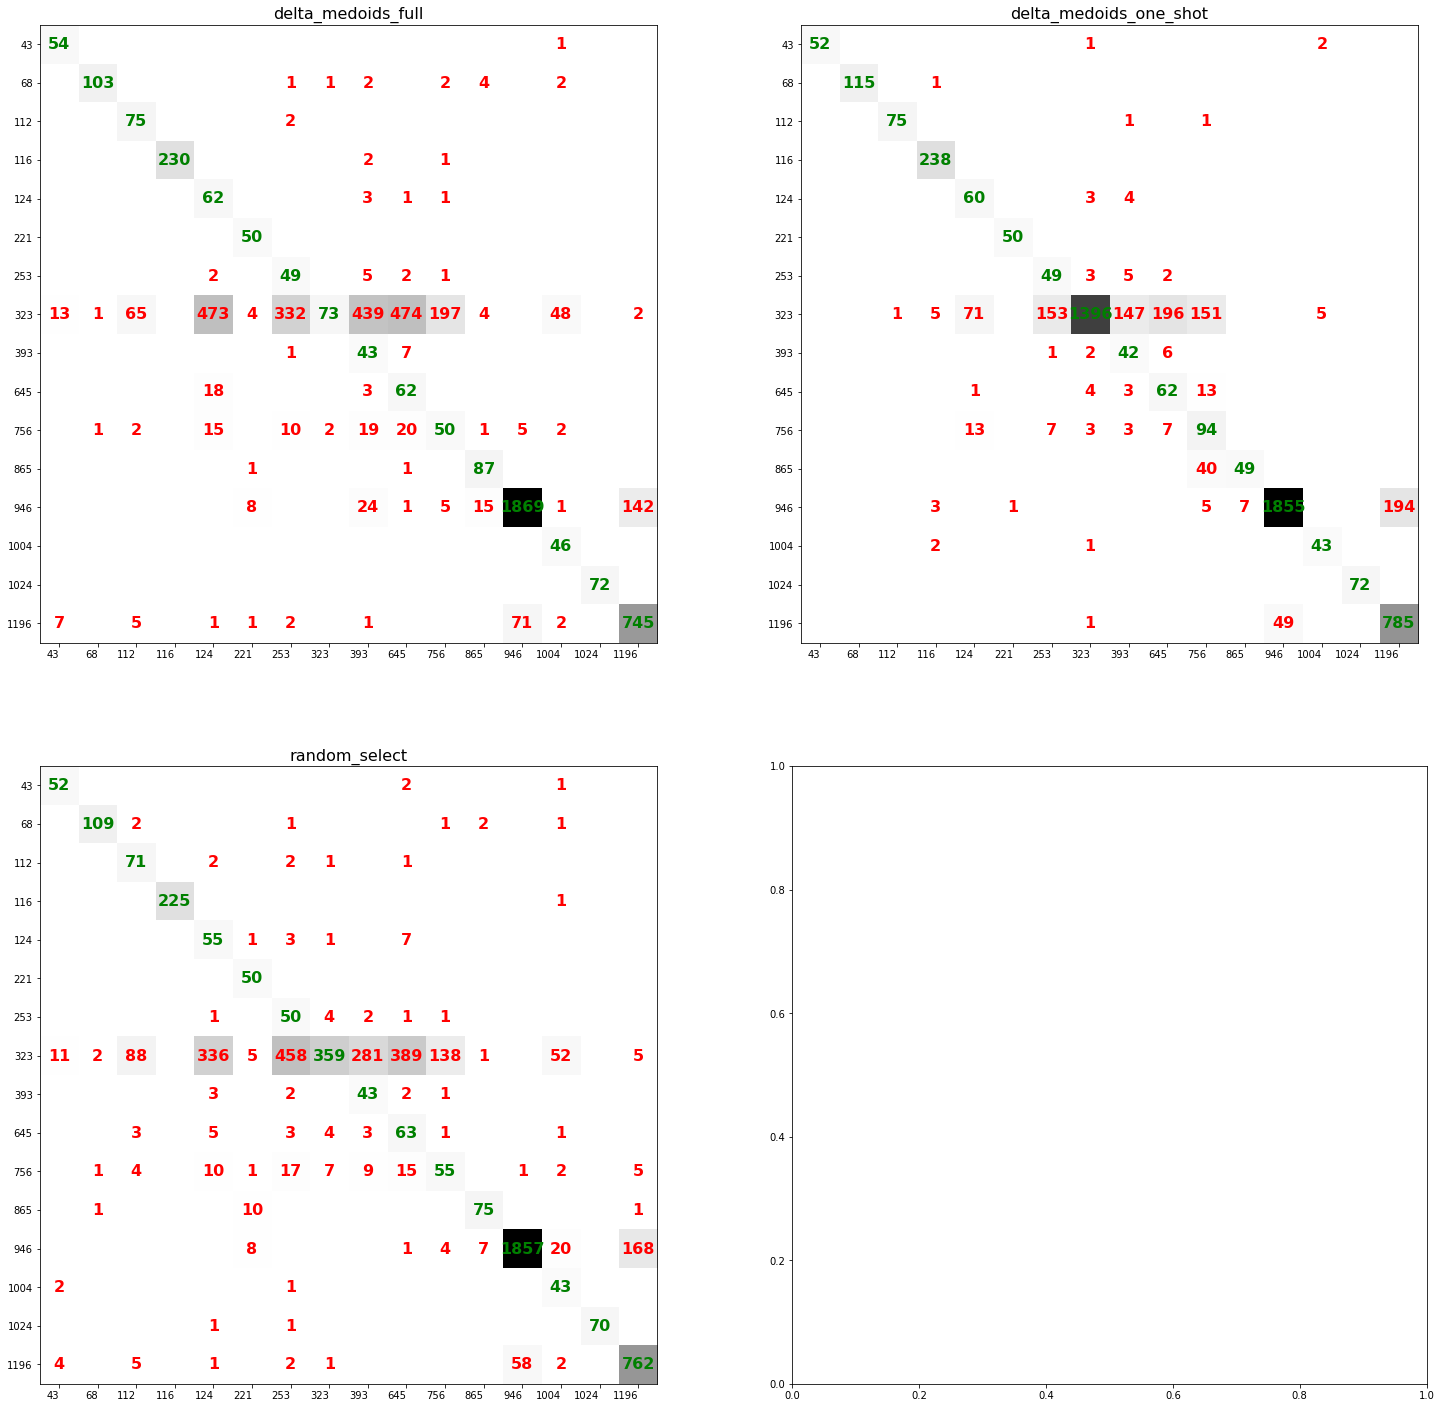
\includegraphics[width=\linewidth]{img/exp4.png}
  \caption{Confusion matrices for real network data}
  \label{img:exp4}
\end{figure}

For $\delta$-Medoids One Shot 77\% of samples were classified correctly.
Such a high percentage is given by the fact, that the algorithm selects sometimes even more than half of the dataset.
For Random Selection this percentage is 63\%.
The $\delta$-Medoids Modified algorithm surpassed it at 79\% of samples correctly assigned to their cluster in classification.

\subsection{Conclusion for Network Security Dataset}
The results show that the $\delta$-Medoids algorithm is better than selecting random representatives from the cluster.
The classification routine was able to classify most of the test samples correctly with it.
The performance improvement can be seen in a complex cluster H.
The $\delta$-Medoids algorithm was able to represent it the best.
Even for clusters with several thousands of samples, few samples were selected a while retaining dominant properties for assigning points to clusters properly.

Another good result is that the $\delta$-Medoids Modified algorithm gives the means to find the number of representatives needed to represent the cluster.
In random selection, a constant is needed which is hard to guess without prior knowledge about the cluster.
For some clusters, 20 representatives might be enough, and for others, a higher number might be needed.
Selecting the higher number to be safe leads to unwanted computational overhead.

\section{Fit of the Data}\label{sec:exp5}

In this experiment the data fit as defined in Section~\ref{sec:representative_selection} was tested.
The motivation was to test how many samples are covered by each added sample and whether on average the $\delta$-Medoids algorithm performs better than Random Selection algorithm.

\subsection{Experimental Setup}
In this experiment, one complex cluster (cluster K) from Network Security Dataset was represented by $\delta$-Medoids and Random Selection algorithms.
After the representatives were selected, the percentage of coverage by each representative was calculated and plotted into a graph.

\subsection{Results}
Figure~\ref{img:exp5} shows the fit of representatives selected from cluster K.

\begin{figure}[t]
  \includegraphics[width=\linewidth]{img/exp5-usable.png}
  \caption{Average fit of representatives in one cluster}
  \label{img:exp5}
\end{figure}

\subsection{Conclusion for Fitting the Data}
On average, the $\delta$-Medoids algorithm covers the cluster better with each added representative.
In the random selection, there is the possibility of selecting either the border cases or two points with overlapping neighborhoods.
This can occur even more often in data, that do not have standard distribution and can be denser in one part of a cluster than the other.

\setsecnumdepth{part}

%========================================CHAPTER==================================

\chapter{Conclusion}

Methods that are relevant for creating cluster prototypes in a non-metric space were studied.
Several methods including Random Selection, Greedy Selection and $\delta$-Medoids algorithms were chosen as relevant.
Furthermore, a new algorithm $\delta$-Medoids Modified was introduced by modifying the $\delta$-Medoids Full algorithm.
Implementation of each algorithm was written and tested on artificially created benchmark datasets.
All algorithms were then further tested on image recognition datasets Pendigits and MNIST Fashion.
Finally, the methods were fine-tuned and tested on a real Network Security Dataset captured in a medium-sized company.

The results presented in this thesis show that the modification made on $\delta$-Medoids Full improves its performance on network security datasets.
The $\delta$-Medoids Modified algorithm can find a small number of representatives with decent coverage of the whole dataset.
It is also able to choose the number of representatives based on the properties of the cluster rather than just guessing the right number of representatives, which is what happens in Random Selection.
Representatives selected this way to fit the dataset on average better than selecting them randomly, which is the method currently used.

The method to represent clusters in non-metric space by a small subset of the whole cluster was implemented and tested in this thesis.
This method was adjusted so that it can be incorporated into Cognitive Targeted Anomaly Detection Framework in the future.

\todo{jak zminit possible future work s kNN graphs atd.}
\todo{zlepseni algoritmu ho zrychlilo}

%\bibliographystyle{iso690}
%\bibliography{hlavac-thesis.bib} \todo{check bibliography correctness}
\begin{thebibliography}{99}
\bibitem{hron2018breaches}
HRON, Martin. The 10 Biggest Data Breaches in 2018. In: \textit{Avast Blog} [online]. Avast Software s.r.o., 2018. [2019-04-05]. Avaiable at: \url{https://blog.avast.com/biggest-data-breaches}

\bibitem{mukherjee1994network}
MUKHERJEE, Biswanath; HEBERLEIN, L. Todd; LEVITT, Karl N. Network intrusion detection. \textit{IEEE network}, 1994, 8.3: 26-41.

\bibitem{cooper2019bestids}
COOPER, Stephen. 2019 Best Intrusion Detection Systems (10+ IDS Tools Reviewed). In: \textit{comparitech} [online]. Comparitech Limited, 2019. [2019-04-27]. Available from: \url{https://www.comparitech.com/net-admin/network-intrusion-detection-tools/}

\bibitem{liao2013intrusion}
LIAO, Hung-Jen, et al. Intrusion detection system: A comprehensive review. \textit{Journal of Network and Computer Applications}, 2013, 36.1: 16-24.

\bibitem{ref2722}
BROWNLEE, N.; MILLS, C.; RUTH, G. Traffic Flow Measurement: Architecture. RFC 2722, October 1999.

\bibitem{grill2016combining}
GRILL, Martin. \textit{Combining network anomaly detectors}. Praha, 2016. Doctoral Thesis. Czech Technical University in Prague. PEVNÝ, Tomáš; REHÁK, Martin.

\bibitem{kopp2018community}
KOPP, Martin; GRILL, Martin; KOHOUT, Jan. Community-based anomaly detection. In: \textit{2018 IEEE International Workshop on Information Forensics and Security (WIFS)}. IEEE, 2018. p. 1-6.

\bibitem{guttag2016introduction}
GUTTAG, John. \textit{Introduction to Computation and Programming Using Python: With Application to Understanding Data}. Second. Cambridge, MA: MIT Press, 2016. ISBN 978-0-262-52962-4.

\bibitem{choudhary1992elements}
CHOUDHARY, B. \textit{The Elements of Complex Analysis}. New Age International, 1993. ISBN 9788122403992.

\bibitem{stahl2014introduction}
STAHL, Saul and Catherine STENSON. \textit{Introduction to Topology and Geometry} [online]. Somerset: John Wiley \& Sons, Incorporated, 2014. ISBN 9781118108109.

\bibitem{tan2014introduction}
TAN, Pang-Ning; STEINBACH, Michael; KUMAR, Vipin. \textit{Introduction to data mining}. Harlow: Pearson, 2014. ISBN 9781292026152.

\bibitem{liebman2015representative}
LIEBMAN, Elad; CHOR, Benny; STONE, Peter. Representative Selection in Nonmetric Datasets. \textit{Applied Artificial Intelligence}, 2015, 29.8: 807-838.

\bibitem{scikit-learn}
PEDREGOSA, Fabian, et al. Scikit-learn: Machine learning in Python. \textit{Journal of machine learning research}, 2011, 12.Oct: 2825-2830.

\bibitem{dua1998pendigit}
Dua, D.; Graff, C. UCI Machine Learning Repository. 2017. Available from: \url{http://archive.ics.uci.edu/ml}

\bibitem{xiao2017fashion}
XIAO, Han; RASUL, Kashif; VOLLGRAF, Roland. Fashion-mnist: a novel image dataset for benchmarking machine learning algorithms. \textit{arXiv preprint arXiv:1708.07747}, 2017.

\bibitem{mckinney2010data}
MCKINNEY, Wes, et al. Data structures for statistical computing in python. In: \textit{Proceedings of the 9th Python in Science Conference}. 2010. p. 51-56.

\end{thebibliography}

\setsecnumdepth{all}
\appendix

\chapter{Abreviations}
% \printglossaries
\begin{description}
%VH I changed the order of NBAD and NIDS to keep alphabetical order
    \item[AD] Anomaly Detection
    \item[DDoS] Distributed Denial of Service
    \item[DPI] Deep Packet Inspection
    \item[IDS] Intrusion Detection System
	\item[NBAD] Network-Based Anomaly Detection
	\item[NIDS] Network Intrusion Detection System
    \item[RFC] Request for Comments
\end{description}


\chapter{Contents of enclosed CD}

%change appropriately

\begin{figure}
	\dirtree{%
		.1 readme.txt\DTcomment{the file with CD contents description}.
		.1 exe\DTcomment{the directory with executables}.
		.1 src\DTcomment{the directory of source codes}.
		.2 wbdcm\DTcomment{implementation sources}.
		.2 thesis\DTcomment{the directory of \LaTeX{} source codes of the thesis}.
		.1 text\DTcomment{the thesis text directory}.
		.2 thesis.pdf\DTcomment{the thesis text in PDF format}.
		.2 thesis.ps\DTcomment{the thesis text in PS format}.
	}
\end{figure}

\end{document}
